%%%%%%%%%%%%%%%%%%%%%%%%%%%%%%%%%%%%%%%%%%%%%%%%%%%%%%%%%%%%%%%%%%%%%%%%
% Copyright (c) 2025 The authors
%
% This work is licensed under a
% Creative Commons Attribution-ShareAlike 4.0 International License.
%
% You should have received a copy of the license along with this
% work. If not, see <http://creativecommons.org/licenses/by-sa/4.0/>.
%%%%%%%%%%%%%%%%%%%%%%%%%%%%%%%%%%%%%%%%%%%%%%%%%%%%%%%%%%%%%%%%%%%%%%%%


%%%%%%%%%%%%%%%%%%%%%%%%%%%%%%%%%%%%%%%%%%%%%%%%%%%%%%%%%%%%%%%%%%%%%%%%%%
%% Supplementary material
%%%%%%%%%%%%%%%%%%%%%%%%%%%%%%%%%%%%%%%%%%%%%%%%%%%%%%%%%%%%%%%%%%%%%%%%%%

\section{Model choice and implementation details}\label{app:model-choice}

\subsection{Posterior distributions}\label{app:posterior}

For the posterior distributions in our Bayesian formulation, we only compute a function proportional to their log-density, since that is enough for a MCMC algorithm to work. Consider the parameter vector \((p, \theta_p)\), where \(\theta_p=(b_p, \tau_p, \alpha, \sigma^2)\) with \(b_p=(\beta_1, \dots, \beta_p)\) and \(\tau_p = (t_1,\dots, t_p)\). Recall that we have a labeled data set of independent observations from \((X, Y)\), denoted by \(\mathcal D_n =\{(X_i, Y_i): i=1,\dots, n\}\). A standard algebraic manipulation in the posterior expression using Bayes' formula yields the following results.

\begin{proposition} Under the linear RKHS model and the prior distribution in Section~\ref{sec:rkhs-linear-model}, the log-posterior distribution up to an additive constant is
  \begin{align*}
  \log\Pi_n(p, \theta_p\mid \mathcal D_n) \propto {} & -\frac{1}{2}\left(\frac{\|b_p\|^2}{\eta^2} - \frac{\|\bm{Y}_n - \alpha\bm{1}_n + \mathcal X_{\tau_p} b_p\|^2}{\sigma^2} \right) - (n+2)\log \sigma\\
  &- p\log \eta - \frac{p}{2}\log(2\pi) + \log \Pi(p),
  \end{align*}
  where \(\bm Y_n=(Y_1,\dots,Y_n)^T\), \(\bm{1}_n\) is an \(n\)-dimensional vector of ones, and \(\mathcal X_{\tau_p}\) is the data matrix \((X_i(t_j))_{i,j}\), for \(i=1,\dots,n\) and \(j=1,\dots,p\).
\end{proposition}

\begin{proposition}
  Under the logistic RKHS model and the prior distribution in Section~\ref{sec:rkhs-logistic-model}, the log-posterior distribution up to an additive constant is
  \begin{align*}
    \log \Pi_n(p, \theta_p \mid \mathcal D_n) \propto {} & \sum_{i=1}^n \left[Y_i \left(\alpha + \dotprod{X_i}{\beta}_K\right) - \log\left(1 + \exp\left\{\alpha +\dotprod{X_i}{\beta}_K\right\}\right) \right]\\
     & - 3\sum_{j=1}^p \log\left(4\beta_j^2 + 125\right) + p \left[\frac{15}{2}\log 5 + 4 \log 2 - \log (3\pi)\right]\\
     & - \log\left(100 + \alpha^2\right) + \log \Pi(p),
  \end{align*}
  where \(\beta(\cdot)=\sum_{j=1}^p \beta_j K(t_j, \cdot)\) and \(\dotprod{X_i}{\beta}_K = \sum_{j=1}^p \beta_j X_i(t_j)\).
\end{proposition}

The discrete distribution \(\Pi(p)\) used in the experiments is either uniform in \(\{1,\dots, 10\}\), with density \(\Pi_{\text{uniform}}(p)=1/10\), or a Poisson distribution with rate parameter \(\lambda=3\) truncated to \(\{1,\dots, 10\}\), with density
\[
\Pi_{\text{Poisson}}(p) = \frac{3^p}{Cp!}, \quad p\in\{1,\dots,10\},
\]
where the normalization constant is \(C = \sum_{k=1}^{10} \frac{3^k}{k!}\).

\subsection{Label switching}\label{app:label-switching}

A well-known issue that arises when using MCMC methods in mixture-like models such as the one proposed in this work is \textit{label switching}, which in short refers to the non-identifiability of the components of the model caused by their interchangeability. In our case, this happens because the likelihood and the prior are symmetric with respect to the ordering of the parameters \(b\) and \(\tau\), i.e., \(\mathcal L(Y|X,\theta)=\mathcal L(Y|X, \theta[\nu])\) for any permutation \(\nu\) that rearranges the indices \(j=1,\dots, p\). Thus, since the components are arbitrarily ordered, they may be inadvertently exchanged from one iteration to the next in a MCMC algorithm. This can cause nonsensical answers when summarizing the marginal posterior distributions of the parameters to perform inference, as different labelings might be mixed on each component \citep{stephens2000dealing}. This is primarily the reason why we do not directly use summaries of the posterior distribution of the individual parameters in our prediction methods.

Moreover, the use of trans-dimensional samplers exacerbates this problem, since the change in dimension can further disrupt the internal ordering of the components \citep[see][]{roodaki2014relabeling}. However, this phenomenon is perhaps surprisingly a condition for the convergence of the MCMC method: as pointed out by many authors \citep[e.g.][]{celeux2000computational}, a lack of switching would indicate that not all modes of the posterior distribution were being explored by the sampler. For this reason, many ad-hoc solutions revolve around post-processing and relabeling the samples to eliminate the switching effect, but they generally do not prevent it from happening in the first place.

The most straightforward solutions consist on imposing an artificial identifiability constraint on the parameters to break the symmetry of their posterior distributions; see \citet{jasra2005markov} and references therein. A common approach that seems to work well is to simply enforce an ordering in the parameters in question, which in our case would mean requiring for example that \(\beta_i < \beta_j\) for \(i < j\), or the analogous with the times in \(\tau\). We have implemented a variation of this method described in \citet{simola2021approximate}, which works by post-processing the samples and relabeling the components to satisfy the order constraint mentioned above, choosing either \(b\) or \(\tau\) depending on which set of ordered parameters would produce the largest separation between any two of them (suitably averaged across all iterations of the chains). This is an area of ongoing research, and thus there are other, more complex relabeling strategies, both deterministic and probabilistic. A summary of several such methods can be found for example in \citet{sperrin2010probabilistic} or \citet{rodriguez2014label}.

\subsection{Affine-invariant ensemble samplers}\label{app:ensemble-sampler}

An interesting and often desirable property of regular MCMC sampling algorithms is that they be \textit{affine-invariant}, which informally means that they regard two distributions that differ in an affine transformation, say \(\pi(x)\) and \(\pi_{A, b}(Ax + b)\), as equally difficult to sample from. This is useful when one is working with very asymmetrical or skewed distributions, for an affine transformation can turn them into ones with simpler shapes. Generally speaking, a MCMC algorithm can be described through a function \(R\) as \(\Lambda(t+1)=R(\Lambda(t), \xi(t), \pi)\), where \(\Lambda(t)\) is the state of the chain at instant \(t\), \(\pi\) is the objective distribution, and \(\xi(t)\) is a sequence of i.i.d.\ random variables that represent the random behavior of the chain. With this notation, the affine-invariance property can be characterized as \(R(A\lambda+b, \xi(t), \pi_{A,b}) = AR(\lambda, \xi(t), \pi) + b\), for all \(A,b\) and \(\lambda\), and almost all \(\xi(t)\). This means that if we fix a random generator and run the algorithm twice, one time using \(\pi\) and starting in \(\Lambda(0)\) and a second time using \(\pi_{A,b}\) with initial point \(\Gamma(0)=A\Lambda(0)+b\), then \(\Gamma(t)=A\Lambda(t)+b\) for all \(t\). In \citet{goodman2010ensemble} the authors consider an ensemble of samplers with the affine invariance property. Specifically, they work with a set \(\Lambda=(\Lambda_1, \dots, \Lambda_L)\) of \textit{walkers}, where \(\Lambda_l(t)\) represents an individual chain at time \(t\). At each iteration, an affine-invariant transformation is used to find the next point, which is constructed using the current values of the rest of the walkers (similar to Gibb's algorithm), namely the \textit{complementary ensemble}
\[
  \Lambda_{-l}(t) = \{\Lambda_1(t+1), \dots, \Lambda_{l-1}(t+1), \Lambda_{l+1}(t), \dots, \Lambda_L(t)\}, \quad l=1,\dots, L.
\]

To maintain the affine invariance and the joint distribution of the ensemble, the walkers are advanced one by one following a Metropolis-Hastings acceptance scheme. The authors consider mainly two types of moves:

\begin{description}
  \item[Stretch move.] For each walker \(1\leq l \leq L\) another walker \(\Lambda_j \in \Lambda_{-l}(t)\) is chosen at random, and the proposal is constructed as
  \[
    \Lambda_l(t) \to \Gamma = \Lambda_j + Z(\Lambda_l(t) - \Lambda_j),
  \]
  where \(Z \stackrel{i.i.d.}{\sim} g(z)\) satisfying the symmetry condition \(g(z^{-1})=zg(z)\). In particular, the suggested density is
  \[
    g_a(z) \propto \begin{cases}
      \frac{1}{\sqrt{z}}, & \text{if } z \in [a^{-1}, a], \\
      0,                  & \text{otherwise.}
    \end{cases}, \quad a > 1.
  \]
  Supposing \(\R^p\) is the sample space, the corresponding acceptance probability (chosen so that the detailed balance equations are satisfied) is:
  \[
    \alpha = \min\left\{1, \ Z^{p-1}\frac{\pi(\Gamma)}{\pi(\Lambda_l(t))}\right\}.
  \]

  \item[Walk move.] For each walker \(1\leq l \leq L\) a random subset \(S_l \subseteq \Lambda_{-l}(t)\) with \(|S_l| \geq 2\) is selected, and the proposed move is
  \[
    \Lambda_l(t) \to \Gamma = \Lambda_l(t) + W,
  \]
  where \(W\) is a normal distribution with mean \(0\) and the same covariance as the sample covariance of all walkers in \(S_l\). The acceptance probability in this case is just the Metropolis ratio, namely \(\alpha=\min\{1, \pi(\Gamma)/\pi(\Lambda_l(t))\}\).
\end{description}

From a computational perspective, the Python library \textit{emcee} \citep{foreman2013emcee}  provides a parallel implementation of this algorithm. The idea is to divide the ensemble \(\Lambda\) into two equally-sized subsets \(\Lambda^{(0)}\) and \(\Lambda^{(1)}\), and then proceed on each iteration in the following alternate fashion:
\begin{enumerate}
  \item Update \textit{all} walkers in \(\Lambda^{(0)}\) through one of the available moves explained above, using \(\Lambda^{(1)}\) as the complementary ensemble.
  \item Use the new values in \(\Lambda^{(0)}\) to update \(\Lambda^{(1)}\).
\end{enumerate}
In this way the detailed balance equations are still satisfied, and each of the steps can benefit from the computing power of an arbitrary number of processors (up to \(L/2\)).  

\subsection{RJMCMC implementation}

For the computational implementation of our Bayesian prediction pipeline we chose the Python library \textit{Eryn} \citep{karnesis2023eryn}. This package is a general-purpose suite of MCMC methods which is reliable, easy to use and performs well in a wide class of problems. It is an enhancement of the \textit{emcee} library mentioned in Appendix~\ref{app:ensemble-sampler} that implements affine-invariant ensemble samplers, with a few key improvements:

\begin{description}
  \item[Reversible jump sampling.] The main reason for choosing this library is that it implements a reversible jump MCMC sampling scheme, which is an essential element in our proposed methodology. It allows trans-dimensional sampling for posterior approximation, letting the user select the likelihood, prior and proposal distributions, and providing a great level of control over the details.

  \item[Parallel tempering.] This is a mechanism to increase the efficiency with which the sampler explores the parameter space. The basic idea is to consider a set of Markov chains in parallel, each one sampling from a transformed posterior distribution given by \(\pi_T(p, \theta_p|X,Y) = \pi(Y|X, p, \theta_p)^{1/T}\pi(p, \theta_p)\), where \(T\geq 1\) is the temperature. In the words of \citet{karnesis2023eryn}, \textit{``intermediate temperatures `smooth out' the posterior by reducing the contrast between areas of high and low likelihood''}. In practice, these chains periodically exchange information, with the swaps controlled by an acceptance probability that maintains detailed balance, and ultimately we are only interested on the cold chain (\(T=1\)).

  \item[Multiple try.] Since the trans-dimensional moves are harder to manage and generally give a low acceptance rate, this library allows the proposal of several candidates for a given move, using a weight function to assign them a relative importance, and then choosing from them with probability given by the normalized weights. This naturally increases the computational cost, but it often produces better results.
\end{description}

Another advantage of this ensemble approach, apart from the property of affine-invariance, is that it only requires the specification of a few hyperparameters irrespective of the underlying dimension. This contrasts to, say, the \(O(N^2)\) degrees of freedom corresponding to the covariance matrix of an \(N\)-dimensional jump distribution in Metropolis-Hastings. We already covered the prior, likelihood and posterior distributions used in Section~\ref{sec:methodology} and in Appendix~\ref{app:posterior}. We give below an overview of other integral parts of our RJMCMC method with some implementation details.

\subsubsection*{Initial values}

We need to specify the initial values for the parameters of all the chains in our sampler. In general, we set these values by sampling from the prior distribution of the corresponding parameters. However, in the linear case the prior on \((\alpha, \sigma^2)\) is improper, so we use ad-hoc weakly informative distributions for the initial values instead. For \(\alpha\) we consider a normal distribution with mean \(0\) and standard deviation \(10|\bar{Y}_{\text{scaled}}|\), where \(Y_{\text{scaled}}\) is the version of the original data scaled to have standard deviation unity. For \(\sigma^2\) we use an inverse-gamma distribution with shape parameter \(a=2\) and scale parameter \(b=\hat\sigma^2_Y/\operatorname{Var}(Y)\), where \(\hat \sigma^2_Y\) is a rough estimate of an acceptable error in the scale of \(Y\). This estimation is done is practice as two order of magnitudes less than \(|\bar{Y}|\).

\subsubsection*{Moves}

As with any MCMC method, the Markov chains are advanced iteratively through a set of moves. For the \textit{in-model} moves (that is, moves that do not change the dimension), we divide our parameter vector in two parts:

\begin{description}
  \item[Stretch move.] For the parameters \(\alpha\) and \(\sigma^2\), which are common to all sub-models, we use the stretch move explained in Appendix~\ref{app:ensemble-sampler}.
  \item[Group stretch move.] For \(b\) and \(\tau\), we use a variant of the stretch move known as the group stretch move, which was designed as an extension of the original move that can handle reversible jump setups. The main difference is that the random walker \(\Lambda_j\) used to advance the chain is selected from a stationary group that does not change for several iterations (see Section~3.1 in \citealp{karnesis2023eryn} for more information about this move).
\end{description}
In both moves above, the key scaling parameter \(a\) starts with a value of \(2\), and is changed dynamically to guide the sampler towards an acceptance rate of about \(20\%-30\%\), which is within the range usually recommended in the literature \citep[e.g.][]{rosenthal2011optimal}.

For the \textit{between-model} moves (those which change the dimension), we set an equal probability of births and deaths, except on the end points of the range of \(p\). Specifically, \(b_{p,p+1}=d_{p, p-1}=0.5\) if \(1<p<10\), and \(b_{1,2}=d_{10,9}=1\). Note that these are only the probabilities to propose the corresponding move, which will be accepted or rejected according to the acceptance formula in Section~\ref{sec:rjmcmc}. When the birth of a new component is proposed, we use the prior distribution of \(b\) and \(\tau\) to generate the new values, and when a death is proposed, the method selects an existing component at random as a candidate for deletion.

\subsubsection*{Hyperparameters}

Other relevant hyperparameters include the burn-in period for the chains, which is the number of initial samples discarded, the number of actual steps, the number of chains, and the number of temperatures for parallel tempering. In the experiments we use 64 chains and 10 different temperatures, and run them for 5000 iterations in total, discarding the first 4000 as burn-in. Moreover, when the prior on \(p\) is uniform (i.e.~in the experiments with real data) we activate the multiple try scheme and set the number of tries to \(2\). Lastly, a computational decision we made is working with \(\log \sigma\) instead of \(\sigma^2\) so that the domain of this parameter is an unconstrained space, which is a widespread recommendation that helps increase the sampling efficiency.


\newpage
\section{Proofs of posterior consistency}\label{app:proofs}

In this section we complete the theoretical exposition in Section~\ref{sec:consistency} by providing detailed proofs of the stated results.

\subsection{Consistency via Doob's theorem}

For this part, the general strategy will be to apply Doob's theorem (Theorem~\ref{th:doob}) to a subset of the parameter space \(\Theta\), where permutations are suitably taken into account and full identifiability holds, and then extend the conclusions to the whole parameter space. As we will see shortly, save for an eventual permutation, identifiability of the map \(\theta \mapsto P_\theta(X,Y)\) is obtained in the RKHS case when the covariance function \(K\) of the underlying stochastic process is non-degenerate.

\subsubsection*{Proof of Theorem~\ref{th:consistency-doob-linear}}

\textit{Measurability issues}. We first show the measurability of the mapping \(\theta \mapsto P_\theta(X,Y)(A)\) for every measurable set \(A \subseteq \mathcal X \times \mathcal Y\). Define the function \(h(\theta, x, y)=f_\theta(y|x)\bm{1}_A(x,y)\), where \(f_\theta(\cdot|x)\) is the density of the normal distribution \( \mathcal N(\alpha + \sum_j \beta_j x(t_j),\, \sigma^2)\), and \(\bm{1}_{A}\) is the indicator function of the set \(A\). Let \(E(x,t)=x(t)\) be the evaluation map on \(\mathcal C[0,1]\times [0,1]\), and note that \(x\mapsto x(t)\) is continuous on \(\mathcal C[0,1]\) while \(t\mapsto x(t)\) is continuous on \([0,1]\). It follows that \(E\) is a Carathéodory function and hence jointly measurable \citep[][Lemma~4.51]{aliprantis2006infinite}. Thus, \(h\) is seen to be measurable as a composition of Borel measurable functions, and by Tonelli's theorem \citep[e.g.][Theorem~2.37]{folland1999real} the function
\[
  \theta \mapsto \int_{\mathcal X \times \mathcal Y} h(\theta, x, y)\, d\rho = P_\theta(X, Y)(A)
\]
is measurable. Another measurability concern is the existence of regular conditional distributions such as \(\theta|(X, Y)_{1:n}\). For this, one should see Theorem 10.2.1 and Theorem 10.2.2 in \citet{dudley2002real}, which guarantee they are well-defined provided that the underlying spaces are sufficiently regular.

\textit{Reduced parameter space}. Consider the space \(\R_\delta = (-\infty, -\delta]\cup[\delta, +\infty)\), with \(\delta\) the fixed tolerance given in Condition~\ref{cond:condition-ident}-\ref{cond:condition-ident-2}, and define
\[\tTheta_p = \R^p_\delta \times [0,1]^p_{\text{ord}} \times \R \times \R^+_0,
\]
where \(
[0,1]^p_{\text{ord}} =\{(t_1,\dots, t_p) \in [0,1]^p: t_1 < \cdots < t_p\}
\). Now consider \(\tTheta = \bigcup_{p\in \N}\tTheta_p\), and note that the sets \(\tTheta_1,\tTheta_2,\ldots\) are still disjoint. Then, again by Proposition A.1 in \citet{miller2023consistency}, we can conclude that \(\tTheta\) is a complete separable metric space under the metric \(d_\Theta\) in~\eqref{eq:metric-doob}. We will henceforth say that a parameter in \(\tTheta\) is ``ordered''.

\textit{Transformation into ordered form}. For \(\theta\in\Theta_p\), define \(T(\theta)=\theta[\nu]\) if there is a \(\nu\in S_p\) such that \(\theta[\nu]\in \tTheta_p\); otherwise set \(T(\theta)=\theta\). Note that we can only transform \(\theta\) to be in \(\tTheta_p\) if the times \(t_j\) are all distinct and the coefficients \(\beta_j\) satisfy \(|\beta_j|\geq\delta\). But since the prior distribution assigns probability one to both events by Condition~\ref{cond:condition-ident}, we have \(\Pi(T(\theta)\in\tTheta)=1\). It will be useful later to observe that for any set \(B\subseteq \tTheta_p\), if we denote \(B[\nu] = \{\theta[\nu]: \theta \in B\}\), we have
\begin{equation}\label{eq:inverse-image-T}
  \bigcup_{\nu\in S_p} B[\nu] = T^{-1}(B).
\end{equation}

\textit{Collapsed model}. Let \(\tilde \Pi_T\) denote the distribution of \(T(\theta)\) restricted to \(\tTheta\), and note that we have \(P_{T(\theta)}(X,Y)=P_{\theta}(X,Y)\). Then the following model holds on the reduced space \(\tTheta\):
\begin{equation}\label{eq:model-linear-collapsed}
  \begin{aligned}
     & T(\theta) \sim \tilde{\Pi}_T,                                         \\
     & (X,Y)_{1:n}\mid T(\theta) \sim P_{T(\theta)}(X,Y) \quad \text{i.i.d.}
  \end{aligned}
\end{equation}

\textit{Verifying conditions}. We will now show that the conditions of Doob's theorem hold on \(\tTheta\). First, since \(\theta \mapsto P_\theta(X, Y)(A)\) is measurable on \(\Theta\), it is also measurable on \(\tTheta\) for all sets \(A\subseteq \mathcal X \times \mathcal Y\) measurable. For the identifiability part, suppose by contradiction that there are two parameters \(\theta,\theta' \in \tTheta\) such that \(\theta\neq \theta'\) and \(P_{\theta}(X, Y) = P_{\theta'}(X, Y)\). Then necessarily \(P_{\theta}(Y|X) = P_{\theta'}(Y|X)\), which in turn implies that the means and variances of these distributions are equal, i.e., \(\sigma^2=(\sigma^2)'\) and
\[
  \alpha + \sum_{j=1}^{p(\theta)} \beta_j X(t_j) = \alpha' + \sum_{j=1}^{p(\theta')} \beta'_j X(t'_j),
\]
where \(t_j\neq t_k\) and \(t_j'\neq t_k'\) for \(j\neq k\). Reordering the terms and combining those where the impact points coincide, we have a linear combination of marginals of the process \(X\) that equals a constant. By taking variances, we can see that all the coefficients in this linear combination must vanish, since the covariance function of the process is strictly positive definite. But \(\beta_j\) and \(\beta_j'\) cannot be \(0\) for any \(j\) (by definition of \(\tTheta\)), so it must be the case that \(\theta'=\theta[\nu]\) for some \(\nu \in S_p\), where \(p=p(\theta)=p(\theta')\). However, \(t_1< \cdots < t_p\) and \(t'_1 < \cdots < t'_p\), so  \(\nu\) must be the identity permutation, that is, \(\theta'=\theta\), contradicting the initial assumption.

\textit{Applying Doob's theorem}. Next we analyze the conclusions of Doob's theorem applied to the collapsed model~\eqref{eq:model-linear-collapsed}: there exists \(\tTheta_* \subseteq \tTheta\) with \(\Pi(T(\theta)\in\tTheta_*)=1\) such that, if \(T(\theta_0)\in \tTheta_*\) and we have \((X,Y)_{1:\infty} \sim P_{T(\theta_0)}(X, Y)\) i.i.d., then for any neighborhood \(B\subseteq \tTheta\) of \(T(\theta_0)\) it holds that
\begin{equation}\label{eq:consistency-collapsed}
  \Pi_n(T(\theta) \in B \mid (X,Y)_{1:n}) \xrightarrow[]{n\to\infty} 1 \quad P_{T(\theta_0)}^\infty-\text{a.s.}
\end{equation}
Now define \(\Theta_*\) to be the set of all parameters in \(\Theta\) that can be obtained by permuting a parameter in \(\tTheta_*\), i.e., \(\Theta_* = \bigcup_{p=1}^\infty \bigcup_{\nu\in S_p}(\tTheta_* \cap \tTheta_p)[\nu]\). Then, by~\eqref{eq:inverse-image-T} we have
\[
  \Pi(\theta\in \Theta_*) = \Pi\left(T(\theta) \in \bigcup_{p=1}^\infty (\tTheta_*\cap \tTheta_p)\right) = \Pi(T(\theta)\in \tTheta_*) = 1.
\]

\textit{Extending the result to \(\Theta\)}. Let \(\theta_0\in\Theta_*\), suppose that \((X,Y)_{1:\infty}\sim P_{\theta_0}(X, Y)\) i.i.d., and define \(p_0=p(\theta_0)\) and \(S_0 = S_{p_0}\). Fix \(\epsilon\in(0,1)\) and consider the set \(B\) of all ordered parameters that are within \(\epsilon\) of the ordered version of \(\theta_0\), i.e.,
\begin{equation}\label{eq:set-B}
  B = \left\{ \theta \in \tTheta: d_\Theta(T(\theta_0), \theta) < \epsilon \right\}.
\end{equation}
Observe that, since \(\epsilon < 1\), we have \(B\subseteq \tTheta_{p_0}\) by definition of \(d_\Theta\). Moreover, \(\bigcup_{\nu\in S_{0}}B[\nu]\subseteq \tilde{B}(\theta_0, \epsilon)\). Then, again by~\eqref{eq:inverse-image-T}, we can write
\begin{equation}\label{eq:consistency-intermediate}
  \begin{aligned}
    \Pi_n(\theta \in \tilde{B}(\theta_0, \epsilon) \mid (X,Y)_{1:n}) & \geq \Pi_n(\theta \in \bigcup_{\nu\in S_{0}} B[\nu] \mid (X,Y)_{1:n}) \\
                                                                     & = \Pi_n(T(\theta) \in B \mid (X,Y)_{1:n}).
  \end{aligned}
\end{equation}
Now, \(T(\theta_0)\in{\tTheta_*}\) because \(\theta_0\in\Theta_*\), and in that case we know that the collapsed model is consistent at \(T(\theta_0)\). Note that we also have \((X,Y)_{1:\infty} \sim P_{T(\theta_0)}(X, Y)\) i.i.d.\ (since \(P_{\theta_0}=P_{T(\theta_0)}\)), and the set \(B\) in~\eqref{eq:set-B} is a neighborhood of \(T(\theta_0)\) in \(\tTheta\). Then, by~\eqref{eq:consistency-collapsed} we have \(\Pi_n(T(\theta) \in B | (X,Y)_{1:n}) \xrightarrow[]{n\to\infty} 1, \ P_0^\infty (X,Y)-\text{a.s.}\), and this fact together with~\eqref{eq:consistency-intermediate} proves consistency for \(\theta_0\) in the original model~\eqref{eq:model-linear}. Lastly, since \(\epsilon < 1\) implies \(\tilde{B}(\theta_0,\epsilon) \subseteq \Theta_{p_0}\), we have also proved the second assertion of our theorem:
\begin{align*}
  \Pi_n(\mathcal P=p_0\mid (X,Y)_{1:n}) & = \Pi_n(\theta \in \Theta_{p_0}\mid (X, Y)_{1:n})                                 \\
                                        & \geq \Pi_n(\theta \in\tilde{B}(\theta_0,\epsilon) \mid (X,Y)_{1:n})               \\
                                        & \xrightarrow[n\to\infty]{} 1 \quad P_0^\infty (X,Y)-\text{a.s.}\tag*{\(\square\)} % qed symbol
\end{align*}

\subsubsection*{Proof of Proposition~\ref{prop:consistency-lebesgue-linear}}

Define \(\Theta_*\) as in the proof of Theorem~\ref{th:consistency-doob-linear} above. Recall that \(\Pi(\Theta_*)=1\), and observe that
\[
  0=\Pi(\Theta \setminus \Theta_*) = \sum_{p=1}^\infty \Pi(\Theta_p \setminus \Theta_*|\mathcal P = p)\Pi(\mathcal P = p).
\]
Since \(\Pi(\mathcal P = p)> 0\) for all \(p\), we have \(\Pi(\Theta_p\setminus \Theta_*|\mathcal P = p) = 0\) for all \(p\). Now, for \(\nu \in S_p\), let \(\mu^\nu_p\) be the distribution of \(\theta[\nu]|\mathcal P=p\) under the model, and note that \((\Theta_p\setminus \Theta_*)[\nu] = \Theta_p \setminus \Theta_*\) by definition of \(\Theta_*\). Thus, if \(id\) is the identity permutation, for all \(\nu\in S_p\) it holds that
\begin{equation}\label{eq:measure-zero}
  \mu^\nu_p (\Theta_p \setminus \Theta_*) = \mu_p^{id} (\Theta_p \setminus \Theta_*) = \Pi (\Theta_p \setminus \Theta_*\mid\mathcal P = p) =0.
\end{equation}
Lastly, \(\lambda_p \ll \sum_{\nu\in S_p}\mu^\nu_p\) by assumption, where \(\ll\) denotes absolute continuity, and this together with~\eqref{eq:measure-zero} implies that \(\lambda_p(\Theta_p \setminus \Theta_*)=0\). But this is valid for all \(p\in\N\), so we can conclude that the inconsistency set satisfies \(\lambda_\infty(\Theta\setminus \Theta_*) = \sum_{p=1}^\infty \lambda_p(\Theta_p\setminus \Theta_*)=0\), as claimed.\qed{}

\subsubsection*{The case of fixed dimension}

As we said earlier, the proofs above can be modified in a straightforward way to establish consistency when the number of components \(p\) is fixed.

\begin{corollary}
  Assume model~\eqref{eq:model-linear} with a fixed value of \(p\), where \(\Theta_p\) is the (finite-dimensional) parameter space. If Condition~\ref{cond:condition-ident}-\ref{cond:condition-ident-1} holds, then the posterior is consistent at \(\theta_0\in\Theta_p\) with \(\Pi\)-probability one. Moreover, if condition (ii) in Proposition~\ref{prop:consistency-lebesgue-linear} holds as well, then the inconsistency set has Lebesgue measure zero.
\end{corollary}

In this case Doob's theorem applies directly under the sole condition that the times be distinct with prior probability one. The coefficients \(\beta_j\) do not cause a problem for identifiability now, since the dimension of every parameter is the same. Note that by allowing \(\beta_j\) to be zero we can circumvent the fact that the true value of the parameter might not have exactly \(p\) components, as long as \(p\) is larger than the true value \(p(\theta_0)\). Indeed, if \(\theta_0\in\Theta\) with \(p(\theta_0) < p\) and \((X,Y)_{1:\infty} \sim P_{\theta_0}(X,Y)\) i.i.d., then we can find \(\theta_1\in\Theta_p\), which is just \(\theta_0\) completed with zeros, such that \(P_{\theta_0}\)(X, Y) = \(P_{\theta_1}(X,Y)\) and the result holds almost surely.

\subsection{Consistency and contraction rates via Schwartz's theorem}

In what follows, we introduce the notation \(a\lesssim b\) to mean inequality up to a multiplicative positive constant. We write \(g(n)=O(h(n))\) for positive functions \(g\) and \(h\) if there exist \(C,n_0>0\) such that \(g(n)\leq Ch(n)\) for all \(n\geq n_0\). Intuitively, this means that \(g(n)\) is of order smaller than or equal to \(h(n)\), i.e., \(\lim\sup_{n\to\infty} g(n)/h(n) < \infty\). Moreover, we say that \(g(n)=o(h(n))\) if for every \(c>0\) there exists \(n_0\in\mathbb{N}\) such that \(g(n)\leq ch(n)\) for all \(n\geq n_0\). Equivalently, this means that \(g(n)\) grows much slower than \(h(n)\), i.e., \(\lim_{n\to\infty} g(n)/h(n) = 0\).

Additionally, when the process \(X\) is understood as a mapping \(X:\Omega \to \mathcal C[0,1]\), we will make frequent use of the correspondence \(\mathbb E[g(X)]=\mathbb E_{Q_X}[g]\) for a measurable function \(g\) on \(\mathcal C[0,1]\), where the latter quantity is an integral in the Bochner sense. In a similar vein, if \(e_t:\mathcal C[0,1]\to \mathbb R\) is the evaluation functional \(x\mapsto x(t)\), given \(h:\mathbb R \to \mathbb R\) we will denote \(\mathbb E_{Q_X}[h\circ e_t]\) by \(\mathbb E_{Q_X}[h(x(t))]\). In particular, for \(h=id\) we have
\[
  \mathbb E_{Q_X}[x(t)]:=\mathbb E_{Q_X}[e_t]=\mathbb E[e_t(X)]=\mathbb E[X(t)].
\]

Next, we present a collection of standard results on covering numbers that will be extensively used in the subsequent proofs \citep[see e.g.][]{van1996weak}.

\begin{lemma}\label{lemma:covering-number}
  Suppose \(d\) is a distance on the set of densities \(\mathcal F=\{f_\theta: \theta\in\Theta\}\).
  \begin{enumerate}[label=(\roman*)]
    \item If \(\epsilon\leq \epsilon'\) then \(N(\epsilon', \mathcal F, d) \leq N(\epsilon, \mathcal F, d)\).
    \item If \(d'\) is another distance on \(\mathcal F\) such that \(d\leq \tilde C d'\), then \(N(\epsilon, \mathcal F, d) \leq N(\epsilon/\tilde C, \mathcal F, d')\) for all \(\epsilon > 0\).
    \item If there is a constant \(\tilde C>0\) such that \(d(f_{\theta}, f_{\theta'})\leq \tilde C \|\theta - \theta'\|\) for every \(\theta, \theta' \in  \Theta\), then the corresponding covering numbers satisfy \(N(\epsilon, \mathcal F, d)\leq N(\epsilon/\tilde C, \Theta, \|\cdot\|)\) for all \(\epsilon > 0\). % Theorem 2.7.17 in van der Vaart and Wellner (1996)
    \item If \(\Theta_p \subset \R^p\) has finite diameter \(R_p\), then \(N(\epsilon, \Theta_p, \|\cdot\|) \leq (3R_p/\epsilon)^p\) for all \(0<\epsilon<R_p\). % Proposition C.2 in Ghosal and van der Vaart (2017)
  \end{enumerate}
\end{lemma}

Recall that our full parameter space is the infinite union \(\Theta=\bigcup_{p\in\N}\Theta_p\). As we said in Section~\ref{sec:consistency-schwartz}, for convenience we take the finite-dimensional sets \(\Theta_p\) to be compact spaces. More specifically, we work with
\[
  \Theta_p = \{(b, \tau, \alpha, \sigma^2): b\in [-M_B, M_B]^p, \tau \in [0,1]^p, \alpha\in [-M_A, M_A], \sigma^2 \in [\sigma^2_{\text{min}}, \sigma^2_{\text{max}}]\},
\]
where \(M_A,M_B>0\) and \(0<\sigma^2_{\text{min}}<\sigma^2_{\text{max}}\). For a given parameter \(\theta\in\Theta\) we consider the function \(\mu_\theta:\mathcal C[0,1]\to\mathbb R\) given by \(\mu_\theta(x)=\alpha + \sum_{j=1}^{p(\theta)} \beta_j x(t_j)\), which allows us to express the density of \(Y|X=x, \theta\) in our linear model as the normal density
\[
  f_\theta(y\mid x) = \frac{1}{\sqrt{2\pi\sigma^2}}\exp\left\{-\frac{(y-\mu_\theta(x))^2}{2\sigma^2}\right\}.
\]

\subsubsection*{Proof of Theorem~\ref{th:consistency-schwartz-linear}}

We need to verify the conditions of Theorem~\ref{th:consistency-hellinger}. As was previously announced, we will be using the sieve of parameters \(\Theta_n = \bigcup_{p=1}^{p_n} \Theta_p\), and the corresponding sieve of densities \(\mathcal F_n=\{f_\theta\in \mathcal F: \theta \in \Theta_n\}\). The idea is to select a suitable growth order for the upper limit \(p_n\) in the sieve so that all conditions hold.

\noindent\textit{Condition (i): bounding the metric entropy}

\noindent First, we claim that there exists \(C^{(p)}>0\) so that \(d_H(f_\theta, f_{\theta'})\leq C^{(p)}\|\theta - \theta'\|\) for all \(\theta, \theta'\) in a fixed (finite-dimensional) \(\Theta_p\). Starting with the function \(\mu_\theta\) and a given trajectory \(x\) of \(X\), rewrite the absolute difference in means as
\[
  |\mu_\theta(x) - \mu_{\theta'}(x)| = \left| (\alpha - \alpha') + \sum_{j=1}^p \left(\beta_j (x(t_j) - x(t'_{j}))+ (\beta_j - \beta'_{j})x(t'_{j})\right) \right|.
\]
Now from the triangle inequality, the Cauchy-Schwarz inequality and the fact that \((a+b)^2 \leq 2(a^2 + b^2)\), the following holds \(Q_X\)-a.s.:
\[
  \frac{1}{2}(\mu_\theta(x) - \mu_{\theta'}(x))^2 \leq (\alpha - \alpha')^2 + 2p\left(M_B^2\sum_{j=1}^p |x(t_j) - x(t_j')|^2 + \sum_{j=1}^p x(t'_j)^2|\beta_j - \beta'_j|^2\right).
\]
Note that \(\|\theta-\theta'\|^2\) is always bigger than the sum of just some of the squared components of \(\theta - \theta'\). Using the Lipschitz property in Condition~\ref{cond:condition-schwartz-X} and integrating on both sides with respect to \(Q_X\), we get
\[
  \frac{1}{2}\mathbb E_{Q_X}\left[(\mu_\theta - \mu_{\theta'})^2\right] \leq \|\theta - \theta'\|^2 + 2p\left(M_B^2 \|\theta - \theta'\|^2 \mathbb{E}_{Q_X}[L^2] + \|\theta - \theta'\|^2 \sup_{t\in[0,1]} \mathbb{E}_{Q_X}[x(t)^2] \right).
\]
Recall that the covariance function \(K\) of \(X\) is assumed to be continuous, so the quantity \(\sup_{t\in[0,1]} \mathbb{E}_{Q_X}[x(t)^2]=\sup_{t\in[0,1]}K(t,t)\) is finite, and so is the integral \(\mathbb{E}_{Q_X}[L^2]\) owing to Condition~\ref{cond:condition-schwartz-X}. Then, we can bring all constants together (which are positive and depend on \(M_B\), \(p\) and \(X\)) into \(C_1>0\) to write
\begin{equation}\label{eq:th9-bound1}
  \mathbb{E}_{Q_X}\left[(\mu_\theta - \mu_{\theta'})^2\right] \leq C_1 \|\theta - \theta'\|^2.
\end{equation}

Now we compute \(d^2_H(f_\theta, f_{\theta'})\). Denote by \(\sigma^2_1\) and \(\sigma^2_2\) the variance parameters corresponding to \(\theta\) and \(\theta'\), respectively. Using the inequality \(e^{-a}\geq 1-a\) for \(a\geq 0\) and the well-known expression for the Hellinger distance between two univariate normal distributions \citep[e.g.][p.~51]{pardo2018statistical}, we have
\begin{align}\label{eq:th9-bound2}
  d^2_H(f_\theta, f_{\theta'}) & = 1 - \int \left(\int\sqrt{f_\theta(y|x) f_{\theta'}(y|x)}\, d\lambda(y)\right) dQ_X(x) \notag                                                                                                                                \\
                               & = 1 - \sqrt{\frac{2\sigma_1\sigma_2}{\sigma_1^2 + \sigma_2^2}}\bigintssss \exp\left\{ -\frac{(\mu_\theta(x) - \mu_{\theta'}(x))^2}{4(\sigma_1^2 + \sigma_2^2)} \right\} dQ_X(x) \notag                                        \\
                               & \leq 1 - \sqrt{\frac{2\sigma_1\sigma_2}{\sigma_1^2+\sigma_2^2}} + \sqrt{\frac{2\sigma_1\sigma_2}{\sigma_1^2 + \sigma_2^2}} \bigintssss \frac{(\mu_\theta(x) - \mu_{\theta'}(x))^2}{4(\sigma_1^2+\sigma_2^2)}\, dQ_X(x) \notag \\
                               & \leq C_2\|\theta - \theta'\|^2 + C_3 \mathbb E_{Q_X}\left[(\mu_\theta - \mu_{\theta'})^2\right],
\end{align}
where \(C_2\) and \(C_3\) are positive constants that depend on \(\sigma^2_{\text{min}}\) and \(\sigma^2_{\text{max}}\). Obtaining \(C_3\) is straightforward; to get \(C_2\), let \(u=\sigma_1^2\), \(v=\sigma_2^2\) and \(S=\sqrt{\frac{2\sqrt{uv}}{u+v}}\), and note that
\[
  1 - \sqrt{\frac{2\sigma_1\sigma_2}{\sigma_1^2 + \sigma_2^2}} = 1-S = \frac{1-S^2}{1+S} \leq 1 - S^2.
\]
Now, a bit of algebraic manipulation yields
\begin{equation}\label{eq:th9-computation-S}
  1 - S^2 = 1 - \frac{2\sqrt{uv}}{u+v} = \frac{(\sqrt{u}-\sqrt{v})^2}{u+v} = \frac{(u-v)^2}{(u+v)(\sqrt{u} + \sqrt{v})^2},
\end{equation}
and after reverting the change of variables the denominator can be easily bounded in terms of \(\sigma^2_{\text{min}}\) and \(\sigma^2_{\text{max}}\). To conclude, combine~\eqref{eq:th9-bound2} with the previous bound~\eqref{eq:th9-bound1} to get the desired inequality
\begin{equation}\label{eq:th9-bound3}
  d^2_H(f_\theta, f_{\theta'}) \leq C^{(p)} \|\theta - \theta'\|^2,
\end{equation}
where \(C^{(p)}>0\) increases linearly with \(p\).

Next, consider the distance \(d_\Theta\) on \(\Theta\) given in~\eqref{eq:metric-doob}. From~\eqref{eq:th9-bound3} one can readily verify that the Hellinger distance satisfies \(d_H(f_\theta, f_{\theta'}) \leq C(n) d_\Theta(\theta, \theta')\) for \(\theta, \theta' \in \Theta_n\), where \(C(n)=O(p_n)\). Moreover, the relationship \(d_\Theta(\theta,\theta')\leq \|\theta - \theta'\|\) always holds on \(\Theta_p\). Denote by \(R_p\) the diameter of \((\Theta_p, \|\cdot\|)\), and note that each \(\Theta_p\) is contained in a hypercube of dimension \(2p+2\) and length independent of \(p\), say \(\ell\). Then, \(R_p\leq \ell\sqrt{2p+2}\) for all \(p\). Putting it all together and invoking Lemma~\ref{lemma:covering-number}, for sufficiently small \(\epsilon>0\) we have
\begin{align*}
  N(\epsilon, \mathcal F_n, d_H) & \leq N(\epsilon/C(n), \Theta_n, d_\Theta)                               \\
                                 & \leq \sum_{p=1}^{p_n} N(\epsilon/C(n), \Theta_p, \|\cdot\|)             \\
                                 & \leq p_n \left(\frac{3C(n)\ell\sqrt{2p_n+2}}{\epsilon}\right)^{2p_n+2}.
\end{align*}
Taking logarithms, we may write
\begin{equation}\label{eq:th9-bound-covering}
  \log N(\epsilon, \mathcal F_n, d_H) \leq \log p_n + (2p_n+2) \log\left(\frac{3C(n) \ell\sqrt{2p_n+2}}{\epsilon}\right).
\end{equation}
Since \(C(n)=O(p_n)\), it suffices to choose \(p_n\) so that \(p_n\log p_n = o(n)\), or equivalently, \(p_n=o\left(n/\log n\right)\). In this way the right-hand side is eventually less than \(n\epsilon^2\), satisfying the first condition of Theorem~\ref{th:consistency-hellinger}.\\

\noindent\textit{Condition (ii): bounding the prior tail mass}

\noindent We need to show that the tail mass of the prior decays at least exponentially with \(n\). An initial crude bound on this tail mass in the parameter space is
\[
  \Pi(\theta \in \Theta \setminus \Theta_n) = \Pi\left(\theta \in \bigcup_{p=p_n + 1}^\infty \Theta_p\right)  = \sum_{p=p_n+1}^\infty \Pi(\theta \in \Theta_p) \leq \sum_{p=p_n+1}^{\infty} \Pi(p).
\]
Since \(\Pi(p)\lesssim \exp\{-\delta p(\log p)^k\}\) for sufficiently large \(p\) and multiplicative constants do not affect the bound, we can work without loss of generality with \(\Pi(p)=\exp\{-\delta p(\log p)^k\}\). Then, we have
\begin{align*}
  \Pi(\Theta \setminus \Theta_n) & \leq \sum_{p=p_n+1}^\infty \exp\{-\delta p(\log p)^k\}                                \\
                                 & = \sum_{m=1}^\infty \exp\{-\delta (p_n+m)(\log (p_n+m))^k\}                           \\
                                 & \leq \sum_{m=1}^\infty \exp\{-\delta p_n (\log p_n)^k\}\exp\{-\delta m (\log p_n)^k\} \\
                                 & = \exp\{-\delta p_n (\log p_n)^k\} \sum_{m=1}^\infty r_n^m,
\end{align*}
where \(r_n=\exp\{-\delta (\log p_n)^k\}<1\). Summing the geometric series, we get
\begin{equation}\label{eq:proof-infinite-prior-tail-bound}
  \Pi(\Theta \setminus \Theta_n) \leq \exp\{-\delta p_n (\log p_n)^k\} \cdot \frac{\exp\{-\delta (\log p_n)^k\}}{1-\exp\{-\delta (\log p_n)^k\}}.
\end{equation}
Now choose \(p_n \geq \frac{c_1n}{(\log n)^k}\) with \(c_1>0\), and observe that for sufficiently large \(n\) we have
\[
  \log p_n \geq \log(c_1) + \log n - k\log \log n \geq \frac{1}{2}\log n.
\]
In particular, \(p_n\to\infty\). Hence, the fraction in~\eqref{eq:proof-infinite-prior-tail-bound} goes to zero as \(n\) grows, and there exists a constant \(c_2>0\) such that, for large \(n\),
\[
  \frac{\exp\{-\delta (\log p_n)^k\}}{1-\exp\{-\delta (\log p_n)^k\}}\leq c_2.
\]
Then, using the lower bounds on \(p_n\) and \(\log p_n\) it follows that eventually
\begin{align*}
  \Pi(\Theta \setminus \Theta_n) & \leq c_2 \exp\{-\delta p_n (\log p_n)^k\}                                                    \\
                                 & \leq c_2 \exp\left\{-\delta \frac{c_1 n}{(\log n)^k}\left(\frac{1}{2}\log n\right)^k\right\} \\
                                 & = c_2 \exp\left\{-\tilde{C}n\right\}.
\end{align*}
As we said before, multiplicative constants do not significantly affect the bound, so we can absorb \(c_2\) into the exponential. Indeed, observe that \(c_2\leq e^{\xi n}\) for any \(\xi>0\) and \(n\) sufficiently large. Then, we have \(c_2e^{-\tilde{C}n} \leq e^{-(\tilde{C}-\xi)n}\), so it suffices to choose \(\xi\) small enough so that \(C=\tilde{C}-\xi>0\). We still need to translate the bound to the prior on \(\mathcal F \setminus \mathcal F_n\), but this is immediate, since
\[
  \Pi_{\mathcal F}(\mathcal F \setminus \mathcal F_n) = \Pi(\theta\in\Theta: f_\theta \in \mathcal F \setminus \mathcal F_n) \leq \Pi(\Theta \setminus \Theta_n).
\]

Note that the lower bound \(p_n \gtrsim \frac{n}{(\log n)^k}\) does not contradict the upper bound \(p_n=o(n/\log n)\) needed for condition (i) above, so we can choose an appropriate growth rate for \(p_n\) in our sieve to make both conditions hold simultaneously.\\

\noindent\textit{Condition on \(f_0\): verifying the KL support}

\noindent First, we proceed by directly computing \(D_{\mathrm{KL}}(f_0 \,\|\, f_\theta)\) for \(\theta\in\Theta_0\), which again has a familiar formula in the normal case \citep[e.g.][p.~47]{pardo2018statistical}, and bounding the result by a similar bound as in condition (i) above:
\begin{align}\label{eq:th9-bound4}
  D_{\mathrm{KL}}(f_0 \,\|\, f_\theta) & =  \int \left(f_0(y|x)\log\left(\frac{f_0(y|x)}{f_\theta(y|x)}\right)  d\lambda(y)\right)dQ_X(x)  \notag                                                              \\
                                       & = \frac{1}{2}\left(\frac{\sigma_0^2}{\sigma^2} - 1 - \log \frac{\sigma_0^2}{\sigma^2} \right) + \frac{1}{2\sigma^2}\int (\mu_0(x) - \mu_\theta(x))^2\, dQ_X(x) \notag \\
                                       & \leq C_1\|\theta_0 - \theta\|^2 + C_2\|\theta_0-\theta\|^2 \notag                                                                                                           \\
                                       & = \tilde C\|\theta_0 - \theta\|^2.
\end{align}
To obtain \(C_1\), let \(u=\sigma_0^2/\sigma^2\) and \(I=[\sigma^2_{\text{min}}/\sigma^2_\text{max},\, \sigma^2_{\text{max}}/\sigma^2_\text{min}]\), and consider the function \(g(u)=u - 1 - \log u\) for \(u\in I\). Define the auxiliary function \(h(u) = g(u)/(u-1)^2\) for \(u\neq 1\) and \(h(1)=1/2\). It is immediate to show that \(h\) is continuous on \(I\), and thus it attains its maximum value
\[H :=\max_{u \in I} h(u)\geq 1/2 > 0.
\]
It follows that \(g(u) \leq H (u-1)^2\) for \(u\in I\), which gives us the desired bound after undoing the change of variables. Then, from~\eqref{eq:th9-bound4} and the behavior of \(\Pi\) on \(\Theta_0\) we can conclude that \(f_0\in\operatorname{KL}(\Pi_{\mathcal F})\), since for every \(\epsilon>0\) we have
\begin{align*}
  \Pi_{\mathcal F}(f_\theta\in \mathcal F: D_{\mathrm{KL}}(f_0 \,\|\, f_\theta) < \epsilon) & =\Pi(\theta \in \Theta: D_{\mathrm{KL}}(f_0 \,\|\, f_\theta) < \epsilon)      \\
                                                                                            & \geq \Pi(\theta \in \Theta_0: D_{\mathrm{KL}}(f_0 \,\|\, f_\theta) <\epsilon) \\
                                                                                            & \geq \Pi(\theta\in\Theta_0: \|\theta_0 - \theta\|^2 < \epsilon/\tilde C) > 0.
\end{align*}


\subsubsection*{Proof of Theorem~\ref{th:contraction-rate-schwartz-linear}}

We will show that the sequence \(\epsilon_n=Dn^{-\gamma}\) with \(0<\gamma<1/2\) and a certain \(D>0\) satisfies the conditions of Theorem~\ref{th:contraction-rate}, and thus is a posterior contraction rate for our model. Note that the specific value of \(D\) is of no relevance, since it is absorbed into the diverging sequence \(M_n\) in the definition of a contraction rate.

This time we will consider the same type of sieve as before, namely \(\Theta_n = \bigcup_{p=1}^{p_n}\Theta_p\), but with an upper limit given by
\[
  p_n=\left\lfloor\frac{n^{1-2\gamma}}{\log n}\right\rfloor,
\]
where \(\lfloor \cdot \rfloor\) is the floor function. As we will see, the conditions imposed in the statement of Theorem~\ref{th:contraction-rate-schwartz-linear} are precisely the ones needed to ensure that the corresponding sieve of densities \(\mathcal F_n=\{f_\theta\in\mathcal F: \theta \in \Theta_n\}\) satisfies the requirements of Theorem~\ref{th:contraction-rate}.

\noindent\textit{Condition (i): bounding the metric entropy}

\noindent From the reasoning in the proof of Theorem~\ref{th:consistency-schwartz-linear} above (see~\eqref{eq:th9-bound-covering}), we have the bound
\[
  \log N(\epsilon_n/2, \mathcal F_n, d_H)  \leq \log p_n + (2p_n+2)\log\left(\frac{6C(n) \ell\sqrt{2p_n+2}}{\epsilon_n}\right).
\]
Since \(\epsilon_n=Dn^{-\gamma}\), \(C(n)\lesssim  p_n\) eventually, and \(\sqrt{2p_n+2}\leq \sqrt{4p_n}\) for \(p_n\geq 1\), we can absorb all constants inside the second logarithm into \(c_1>0\). Indeed, for sufficiently large \(n\) we have
\begin{equation}\label{eq:th11-bound1}
  \log N(\epsilon_n/2, \mathcal F_n, d_H)  \leq \log p_n + (2p_n+2)\log\left(c_1 p_n^{3/2}n^\gamma\right).
\end{equation}
Then, given that \(p_n\leq \frac{n^{1-2\gamma}}{\log n}\), substituting into~\eqref{eq:th11-bound1} yields
\begin{align*}
  \log N(\epsilon_n/2, \mathcal F_n, d_H) & \leq \log \left(\frac{n^{1-2\gamma}}{\log n}\right)+ \frac{2n^{1-2\gamma}}{\log n}\left[\log c_1 + \log\left(\frac{n^{3/2-2\gamma}}{(\log n)^{3/2}}\right)\right] \\
                                          & \quad + 2\left[\log c_1 + \log\left(\frac{n^{3/2-2\gamma}}{(\log n)^{3/2}}\right)\right].
\end{align*}
Simplifying the expression in the right-hand side, the dominant term for large \(n\) is
\[
  2\left(\frac{3}{2}-2\gamma\right)n^{1-2\gamma} = (3-4\gamma)n^{1-2\gamma},
\]
and the rest of the terms are of order strictly smaller. This means that there exists a constant \(c_2>0\) as small as we want such that every term apart from the dominant term is eventually smaller than \(c_2 n^{1-2\gamma}\). Thus, for sufficiently large \(n\) we can write
\[
  \log N(\epsilon_n/2, \mathcal F_n, d_H)  \leq  (c_2 + 3-4\gamma)n^{1-2\gamma}.
\]
Since \(n\epsilon_n^2 =D^2n^{1-2\gamma}\), the conclusion follows for \(D^2>3-4\gamma\).\\


\noindent\textit{Condition (ii): bounding the prior tail mass}

\noindent We follow a similar reasoning as in the proof of Theorem~\ref{th:consistency-schwartz-linear} above. Consider without loss of generality that \(\Pi(p)=c_1\exp\{-\delta p \log p\}\). Then, we have
\begin{align*}
  \Pi(\Theta \setminus \Theta_n) & \leq \sum_{p>p_n} c_1\exp\{-\delta p \log p\}                                                        \\
                                 & = c_1\sum_{m=1}^\infty \exp\{-\delta (p_n+m) \log(p_n+m)\}                                           \\
                                 & \leq c_1\sum_{m=1}^\infty  \exp\{-\delta(p_n+m)\log p_n\}                                            \\
                                 & \leq c_1\exp\{-\delta p_n \log p_n\} \sum_{m=1}^\infty \left(\exp\{-\delta \log p_n\}\right)^m       \\
                                 & = c_1\exp\{-\delta p_n \log p_n\} \cdot \frac{\exp\{-\delta \log p_n\}}{1-\exp\{-\delta \log p_n\}}.
\end{align*}
Now, since \(p_n\geq \frac{n^{1-2\gamma}}{2\log n}\), for large \(n\) we have
\begin{align*}
  \log p_n & \geq (1-2\gamma)\log n - \log (2\log n) \geq \frac{1-2\gamma}{2}\log n.
\end{align*}
In particular, \(p_n\to\infty\). Hence, there exists a constant \(c_2>0\) such that
\[
  \frac{\exp\{-\delta \log p_n\}}{1-\exp\{-\delta \log p_n\}}\leq c_2
\]
for large \(n\). Then, using the lower bounds on \(p_n\) and \(\log p_n\) it follows that
\[
  \Pi(\Theta \setminus \Theta_n) \leq c_1c_2 \exp\left\{\frac{-\delta (1-2\gamma)}{4}n^{1-2\gamma}\right\}.
\]
At this point we integrate \(c_1c_2\) into the exponential. Let \(c_3=\delta(1-2\gamma)/4>0\) and choose \(0<\xi<c_3\) such that \(c_1c_2\leq \exp\{\xi n^{1-2\gamma}\}\) for sufficiently large \(n\). Then, if \(c_4=c_3-\xi\), we have \(\Pi(\Theta \setminus \Theta_n) \leq \exp\{-c_4n^{1-2\gamma}\}\). Now, observe that \((C+4)n\epsilon_n^2=(C+4)D^2n^{1-2\gamma}\), where \(C\) is the constant appearing in condition (ii) of Theorem~\ref{th:contraction-rate}, so it suffices to choose \(C\leq c_4/D^2 -4\) and we are done. Given the lower bound on \(D\) imposed in condition (i) above, it can be easily verified that this upper bound on \(C\) is positive as long as \(\xi\) is chosen small enough and \(\delta > 16(3-4\gamma)/(1-2\gamma)\), which is true by assumption.\\

\noindent\textit{Condition (iii): sufficient prior mass on \(B_2(f_0, \epsilon_n)\)}

\noindent Let \(\theta\in\Theta_0\). We know from the proof of Theorem~\ref{th:consistency-schwartz-linear} (see~\eqref{eq:th9-bound4}) that there exists a constant \(C_1>0\) such that \(D_{\mathrm{KL}}(f_0 \,\|\, f_\theta)\leq C_1^2 \|\theta_0 - \theta\|^2\). On the other hand, direct calculation \citep[see e.g.][]{choi2007posterior} shows that, under Gaussianity,
\[
  V_2(f_0, f_\theta) = \frac{(\sigma_0^2 - \sigma^2)^2}{2\sigma^4} + \frac{\sigma_0^2}{\sigma^4}\int (\mu_0(x) - \mu_\theta(x))^2\, dQ_X(x).
\]
Following the same reasoning as we did multiple times before, we can see that \(V_2(f_0, f_\theta)\) is bounded above by \(C_2^2\|\theta_0 - \theta\|^2\) with \(C_2>0\). Therefore, if \(\|\theta_0 - \theta\| < \epsilon_n/\tilde C\) where \(\tilde C = \max\{C_1, C_2\}\), it follows that \(D_{\mathrm{KL}}(f_0 \,\|\, f_\theta)< \epsilon_n^2\) and \(V_2(f_0, f_\theta) < \epsilon_n^2\). Thus, if we denote by \(B(\theta_0, \epsilon)\) the open ball of radius \(\epsilon\) centered at \(\theta_0\) in \(\Theta_0\), we have just shown that \(\theta \in B(\theta_0,\epsilon_n/\tilde{C})\) implies \(f_\theta \in B_2(f_0, \epsilon_n)\), and hence
\begin{equation}\label{eq:th11-bound2}
  \Pi_{\mathcal F}(B_2(f_0, \epsilon_n)) \geq \Pi(B(\theta_0,\epsilon_n/\tilde{C})).
\end{equation}

Now, to get the final lower bound required for condition (iii) in Theorem~\ref{th:contraction-rate}, we will use the following auxiliary result.

\begin{lemma}\label{lemma:th11-lemma-lebesgue}
  If the prior \(\Pi\) has a density on \(\Theta_0\) with respect to Lebesgue measure that is bounded away from zero in a neighborhood of \(\theta_0\), then there is a constant \(c>0\) such that \(\Pi(B(\theta_0, r))\geq cr^{2p_0+2}\) for all sufficiently small \(r>0\), where \(p_0=p(\theta_0)\).
\end{lemma}
\begin{proof}
  Let \(g\) be the density of \(\Pi\) restricted to \(\Theta_0\), and let \(r_0>0\) be a radius such that \(g(\theta)\geq g_0>0\) for all \(\theta\in B(\theta_0, r_0)\). Then, for every \(0<r\leq r_0\) we have
  \[
    \Pi(B(\theta_0, r)) =\int_{B(\theta_0, r)} g\, d\lambda_0 \geq g_0 \lambda_0(B(\theta_0, r)) = g_0 c_d r^d,
  \]
  where \(d=2p_0+2\), \(\lambda_0\) is the Lebesgue measure on \(\Theta_0\) and \(c_d>0\) is a constant that depends only on the dimension of \(\Theta_0\).
  \end{proof}
  
  Applying Lemma~\ref{lemma:th11-lemma-lebesgue} with \(r=\epsilon_n/\tilde C=Dn^{-\gamma}/\tilde C\) and taking logarithms in~\eqref{eq:th11-bound2}, we have, for large \(n\),
  \[
  \log \Pi_{\mathcal F}(B_2(f_0, \epsilon_n)) \geq \log c + (2p_0+2)\log\left(\frac{Dn^{-\gamma}}{\tilde C}\right) \geq \tilde c -2\gamma p_0\log n \geq -4\gamma p_0\log n,
  \]
where \(\tilde c > 0\) is an irrelevant constant in the asymptotic regime. To finish the proof we want to find a constant \(C>0\) such that \(\log \Pi_{\mathcal F}(B_2(f_0, \epsilon_n)) \geq - Cn\epsilon_n^2=-CD^2n^{1-2\gamma}\), but \(\log n\) grows much slower than \(n^{1-2\gamma}\), so the inequality \(-4\gamma p_0\log n \geq -CD^2n^{1-2\gamma}\) holds for any choice of \(C>0\) and sufficiently large \(n\).

\subsubsection*{Proof of Corollary~\ref{th:corollary-contraction-rate}}

We simply use the fact that, if \(d\) is another distance on \(\mathcal F\) with \(d\leq \tilde C d_H\), then
\[
  \Pi_n(\theta: d(f_0, f_\theta)>\epsilon\mid \text{data}) \leq \Pi_n(\theta: d_H(f_0, f_\theta)>\epsilon/\tilde C\mid \text{data}).
\]

For the \(L^1\)-distance, by the Cauchy-Schwarz inequality we have
\begin{align*}
  d_1^2(f_0, f_\theta) & = \left(\int |f_0 - f_\theta|\, d\rho\right)^2                                                                          \\
                       & = \left(\int \left|\sqrt{f_0} - \sqrt{f_\theta}\right|\left(\sqrt{f_0} + \sqrt{f_\theta}\right) d\rho\right)^2          \\
                       & \leq \int\left(\sqrt{f_0} - \sqrt{f_\theta}\right)^2 d\rho \cdot \int \left(\sqrt{f_0} + \sqrt{f_\theta}\right)^2 d\rho \\
                       & \leq 8 d^2_H(f_0, f_\theta).
\end{align*}
In the last step we have used the alternative definition of the Hellinger distance, which can be expressed as \(2d_H^2(f_0, f_\theta) = \int\left(\sqrt{f_0} - \sqrt{f_\theta}\right)^2 d\rho \), the basic inequality \((a + b)^2 \leq 2(a^2 + b^2)\), and the fact that both \(f_0\) and \(f_\theta\) integrate to \(1\) over the whole space.

For the mean-variance discrepancy distance, recall the expression for the squared Hellinger distance between two normal densities, which can be formulated in this case as \(d^2_H(f_0, f_\theta)= \int g_{0,\theta}(x)\, dQ_X(x)\), with
\[
  g_{0,\theta}(x) = 1 - \sqrt{\frac{2\sigma_0\sigma}{\sigma_0^2 + \sigma^2}}\exp\left\{ -\frac{(\mu_0(x) - \mu_{\theta}(x))^2}{4(\sigma_0^2 + \sigma^2)} \right\}.
\]
Define \(\Delta_\mu = \mu_0-\mu_\theta\), \(\Delta_{\mu_M} = [\mu_0]_M - [\mu_\theta]_M\) and \(S=\sqrt{\frac{2\sigma_0\sigma}{\sigma_0^2+\sigma^2}}\). On the one hand, using the trivial bounds \(e^{-a}\leq 1\) and \(S\leq 1\), we have
\[
  g_{0,\theta}(x) \geq 1 - S = \frac{1-S^2}{1+S} \geq \frac{1-S^2}{2} \geq C_1(\sigma_0^2 - \sigma^2)^2,
\]
where the last inequality comes from the computations in~\eqref{eq:th9-computation-S}. On the other hand, observe that \(\Delta^2_\mu \geq \Delta^2_{\mu_M}\) and \(\Delta^2_{\mu_M}\leq 4M^2\). Use these facts together with the bound \(1-e^{-a}\geq \frac{a}{1+a}\) for \(a\geq 0\) to get
\[
  g_{0,\theta}(x)  \geq  1 - \exp\left\{ -\frac{\Delta^2_{\mu_M}(x)}{4(\sigma_0^2+\sigma^2)} \right\} \geq C_2\Delta^2_{\mu_M}(x).
\]
Bringing together both pieces of information, we can take \(\tilde C = \min\{C_1, C_2\}\) and write
\[
  g_{0,\theta}(x) \geq \tilde C\left[\Delta^2_{\mu_M}(x) + (\sigma_0^2 - \sigma^2)^2\right],
\]
and integrating on both sides with respect to \(Q_X\) yields
\[
  d_H^2(f_0, f_\theta)\geq \tilde C\left[\|\Delta_{\mu_M}\|^2_{2,Q_X} + (\sigma_0^2 - \sigma^2)^2\right].
\]
To conclude, note that \(\sqrt{a^2+b^2}\geq (1/\sqrt{2})(a+b)\) for \(a,b\geq 0\), so we can take square roots on both sides and get the desired bound.


\subsubsection*{Examples of processes that satisfy Condition~\ref{cond:condition-schwartz-X}}

Condition~\ref{cond:condition-schwartz-X} implies that the process \(X\) is ``mean-square Lipschitz continuous'', i.e., there exists \(L>0\) such that \(\mathbb E[(X(t) - X(s))^2] \leq L (t-s)^2\) for all \(t, s \in [0,1]\). Looking at the derivations we did, we can substitute the almost sure Lipschitzness of the trajectories by this new condition and arrive at the same conclusions. Moreover, note that this guarantees, via Kolmogorov's continuity theorem, that the sample paths of \(X\) (after an eventual modification) are continuous functions. Apart from somewhat trivial examples, such as a deterministic process or a linear random process, we can show that processes with a sufficiently smooth kernel satisfy our requirements.

\begin{lemma}\label{lemma:mean-square-lipschitz}
  If the covariance function \(K\) of the process \(X\) is twice-continuously differentiable and the mean function \(\mathbb E[X(t)]\) vanishes for all \(t\in[0,1]\), then \(X\) is ``mean-square Lipschitz continuous'', that is, there exists \(L>0\) such that \(\mathbb E[(X(t) - X(s))^2] \leq L (t-s)^2\) for all \(t, s \in [0,1]\).
\end{lemma}
\begin{proof}
We know that \(\mathbb E[(X(t) - X(s))^2] = K(t,t)-2K(t,s) + K(s,s)\), and a Taylor expansion around the point \((s,s)\) shows that
\[
  K(t,t)-2K(t,s) + K(s,s) = \partial_{ts}K(s,s)(t-s)^2 + o((t-s)^2).
  \]
Since \(\partial_{ts}K\) is continuous on the compact set \([0,1]^2\), there exists a constant \(L>0\) such that
\[
  K(t,t)-2K(t,s) + K(s,s) \leq L(t-s)^2, \quad \text{for } t\to s.
\]
Lastly, this bound extends to all \(t,s\in[0,1]\) by continuity of \(K\).
% \begin{align*}
%   K(t, t) & = K(s, s) + \partial_1 K(s, s)(t - s) + \partial_2 K(s, s)(t -s)                                                                         \\
%           & + \frac{1}{2}\left[\partial_{11}K(s, s)(t - s)^2 + 2\partial_{12}K(s, s)(t - s)^2 + \partial_{22}K(s, s)(t - s)^2\right] + o((t - s)^2). \\
%   K(t, s) & = K(s, s) + \partial_1 K(s, s)(t - s) + \frac{1}{2}\partial_{11}K(s, s)(t - s)^2 + o((t - s)^2).
% \end{align*}
% Since \(K\) is symmetric, the partial derivatives satisfy \(\partial_{t} K(u,v)= \partial_s K(v,u)\) and \(\partial_{tt} K(u,v)= \partial_{ss} K(v,u)\).
\end{proof}

Note that the above condition is by no means a necessary one. For example, given a zero-mean second-order stochastic process \(\{Z(t): t \in [0,1]\}\), we consider the integrated process
\[
  X(t)=\int_0^t Z(u)\, du, \quad t\in [0,1].
\]
If \(K_Z(t,s)=\mathbb E[Z(t)Z(s)]\) is uniformly bounded above by a constant \(L>0\) on \([0,1]\), we have
\[
  \mathbb E\left[(X(t) - X(s))^2\right] = \int_s^t \int_s^t \mathbb E[Z(u)Z(v)]\, du\,dv \leq L(t-s)^2.
\]
For example, we might take \(Z(t)\) to be a standard Brownian motion, an Ornstein-Uhlenbeck process, or, in general, any second-order process with a continuous covariance function. In any case, by virtue of Lemma~\ref{lemma:mean-square-lipschitz} we can always pre-process the trajectories so that they are smooth enough for the conditions to hold, considering for instance the convolution with a smooth kernel.


\newpage
\section{Experimentation}\label{app:experiments}

\subsection{Overview of data sets and comparison algorithms}\label{app:data-sets}

To generate the simulated data sets for the comparison experiments in Section~\ref{sec:results}, we used four types of Gaussian process regressors commonly employed in the literature, each with a different covariance function:
\begin{description}
  \item [BM.] A Brownian motion, with kernel \(K_1(t,s)=\min\{t,s\}\).
  \item [fBM.] A fractional Brownian motion, with kernel \(K_2(t,s)=1/2(s^{2H} + t^{2H} - |t-s|^{2H})\) and Hurst parameter \(H=0.8\).
  \item [O-U.] An Ornstein-Uhlenbeck process, with kernel \(K_3(t,s)=e^{-|t-s|}\).
  \item [Gaussian.] A Gaussian process with a squared exponential kernel (also known as Gaussian kernel), namely \(K_4(t,s)=e^{-(t-s)^2/2\xi^2}\), where \(\xi=0.2\).
\end{description}

For the comparison algorithms themselves, we considered several frequentist methods which were selected among popular ones in FDA and machine learning in general. As specified earlier, variable selection and dimensionality reduction methods are part of a pipeline followed by a standard multiple regression technique. In the linear regression case, we chose the following algorithms:

\begin{description}
  \item [PLS1.] Partial least squares regression \citep[e.g.][]{abdi2010partial}.
  \item[Lasso.] Linear least squares with \(l^1\) regularization.
  \item [FPLS and FPLS1.] Functional PLS regression through basis expansion, implemented as in \citet{aguilera2010using}.
  \item [FLin.] Standard \(L^2\) functional linear regression model with fixed basis expansion and regularization.
  \item [APLS.] Functional partial least squares regression proposed by \citet{delaigle2012methodology}.
  \item [PLS.] Partial least squares for dimension reduction.
  \item [PCA.] Principal component analysis for dimension reduction.
  \item[Manual.] Dummy variable selection method with a pre-specified number of components (equispaced on \([0, 1]\)).
  \item [FPCA.] Functional principal component analysis.
  \item [Ridge.] Linear least squares with \(l^2\) regularization. This is used as the multiple regression that follows variable selection or dimensionality reduction methods.

\end{description}

In the logistic regression case, all the variable selection and dimension reduction techniques from above were also considered, with the addition of the following classification methods:

\begin{description}
  \item [QDA.] Quadratic discriminant analysis.
  \item [MDC.] Maximum depth classifier \citep[e.g.][]{ghosh2005maximum}.
  \item [Log.] Standard multiple logistic regression with \(l^2\) regularization. This is used as a one-stage method and also as the multiple regression that follows variable selection or dimensionality reduction methods.
  \item [LDA.] Linear discriminant analysis.
  \item [FNC.] Functional nearest centroid classifier with the \(L^2\)-distance.
  \item [FLog.] Functional RKHS-based logistic regression algorithm proposed in \citet{berrendero2023functional}.
  \item [FLDA.] Implementation of the functional version of linear discriminant analysis proposed in \citet{preda2007pls}.
  \item [FKNN.] Functional K-nearest neighbors classifier with the \(L^2\)-distance.
  \item [RKVS.] RKHS-based variable selection and classification method proposed in \citet{berrendero2018use}.
  \item [APLS+NC.] Functional PLS used as a dimension reduction method, as proposed in \citet{delaigle2012achieving} in combination with the nearest centroid (NC) algorithm.
\end{description}

The main hyperparameters of all these algorithms were selected by 10-fold cross-validation, and for those that have a number of components to select, we set 10 as the maximum value so that comparison with our own methods are fair. In particular, regularization parameters are searched among 20 values in the logarithmic space \([10^{-4}, 10^4]\), the number of basis elements for cubic spline bases is in \(\{4,5,\dots,10\}\), the number of basis elements for Fourier bases is one of \(\{1,3,5,7,9\}\), and the number of neighbors in the KNN classifier is in \(\{3,5,7,9,11,13\}\). Most algorithms have been taken from the libraries \textit{scikit-learn} \citep{pedregosa2011scikit} and \textit{scikit-fda} \citep{ramos2024scikit}, the first oriented to machine learning in general and the second to FDA in particular. However, some methods were not found in these packages and had to be implemented from scratch. This is the case of the FLDA, FPLS and APLS methods, which we coded following the corresponding articles.

\subsection{Simulations with non-Gaussian regressors}\label{app:non-gp}

We performed an additional set of experiments in linear and logistic regression in which the regressors are not Gaussian processes (GPs), to see if our methods would hold up in this case. These experiments where run in the same conditions as those reported in Section~\ref{sec:results}.

\subsubsection*{Functional linear regression}

We use a geometric Brownian motion (GBM) as the regressor variable, defined as \(X(t)=\exp\{{\operatorname{BM}(t)}\}\), where \(\operatorname{BM}(t)\) is a standard Brownian motion. In this case we consider two data sets, one with a RKHS response and one with an \(L^2\) response, both with the same parameters as in the corresponding data sets in Section~\ref{sec:results}. The comparison results can be seen in Figure~\ref{fig:reg_non_gp}: in this case our methods still get better results under the RKHS model, while the results under the \(L^2\)-model are essentially the same, which is a positive outcome.

\begin{figure}[ht!]
  \centering
  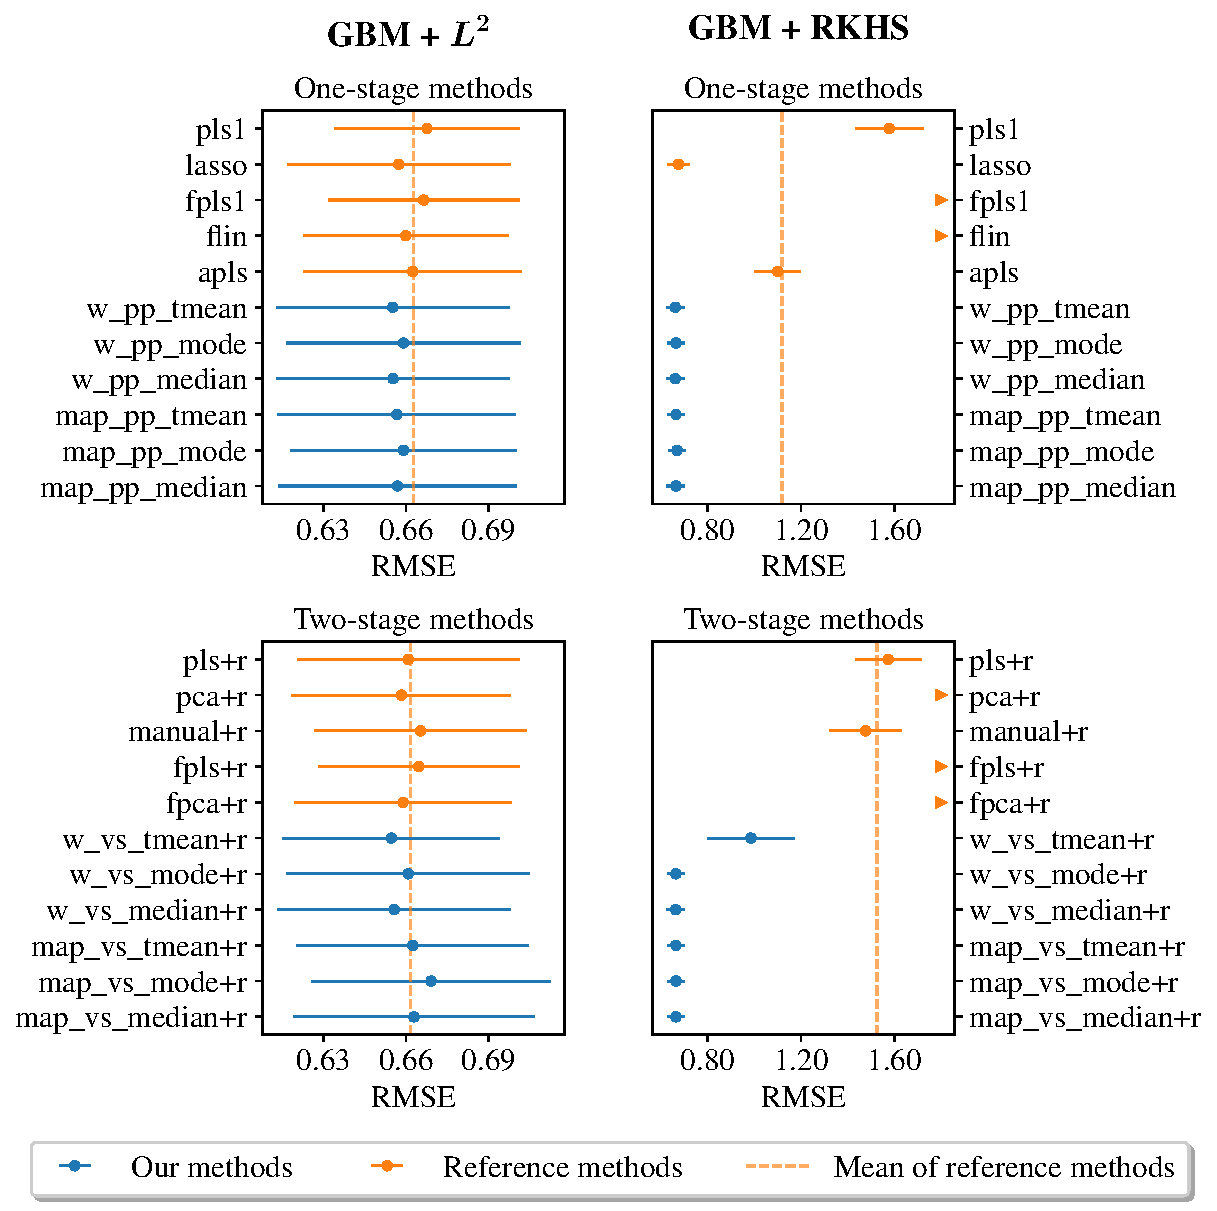
\includegraphics[width=.6\textwidth]{reg_non_gp}
  \caption{Mean and standard error of RMSE of predictors (lower is better) for 10 runs with GBM regressors. In the first column the response obeys a linear \(L^2\)-model, while in the second columns it follows a linear RKHS model.}\label{fig:reg_non_gp}
\end{figure}

\subsubsection*{Functional logistic regression}

We consider a ``mixture'' situation in which we combine regressors from two different GPs with equal probability and label them according to their origin. Firstly, we consider a homoscedastic case to distinguish between a standard Brownian motion and a Brownian motion with a mean function that is zero until \(t=0.5\), and then becomes \(m(t)=0.75t\). Secondly, we consider a heteroscedastic case to distinguish between a standard Brownian motion and a Brownian motion with variance 2, that is, with kernel \(K(t,s)=2\min\{t,s\}\).

Figure~\ref{fig:clf_non_gp} shows that our classifiers perform better than most comparison algorithms in both cases. The differences are most notable in the homoscedastic case, and in the heteroscedastic case the overall accuracy is low. Incidentally, this heteroscedastic case of two zero-mean Brownian motions has a special interest, since it can be shown that the Bayes error is zero in the limit of dense monitoring (i.e.\ with an arbitrarily fine measurement grid), a manifestation of the ``near-perfect'' classification phenomenon analyzed for example in \citet{torrecilla2020optimal}. Our results are in line with the empirical findings of this article, where the authors conclude that even though the asymptotic theoretical error is zero, most classification methods are suboptimal in practice (possibly due to the high collinearity of the data), with the notable exception of PCA+QDA.

\begin{figure}[ht!]
  \centering
  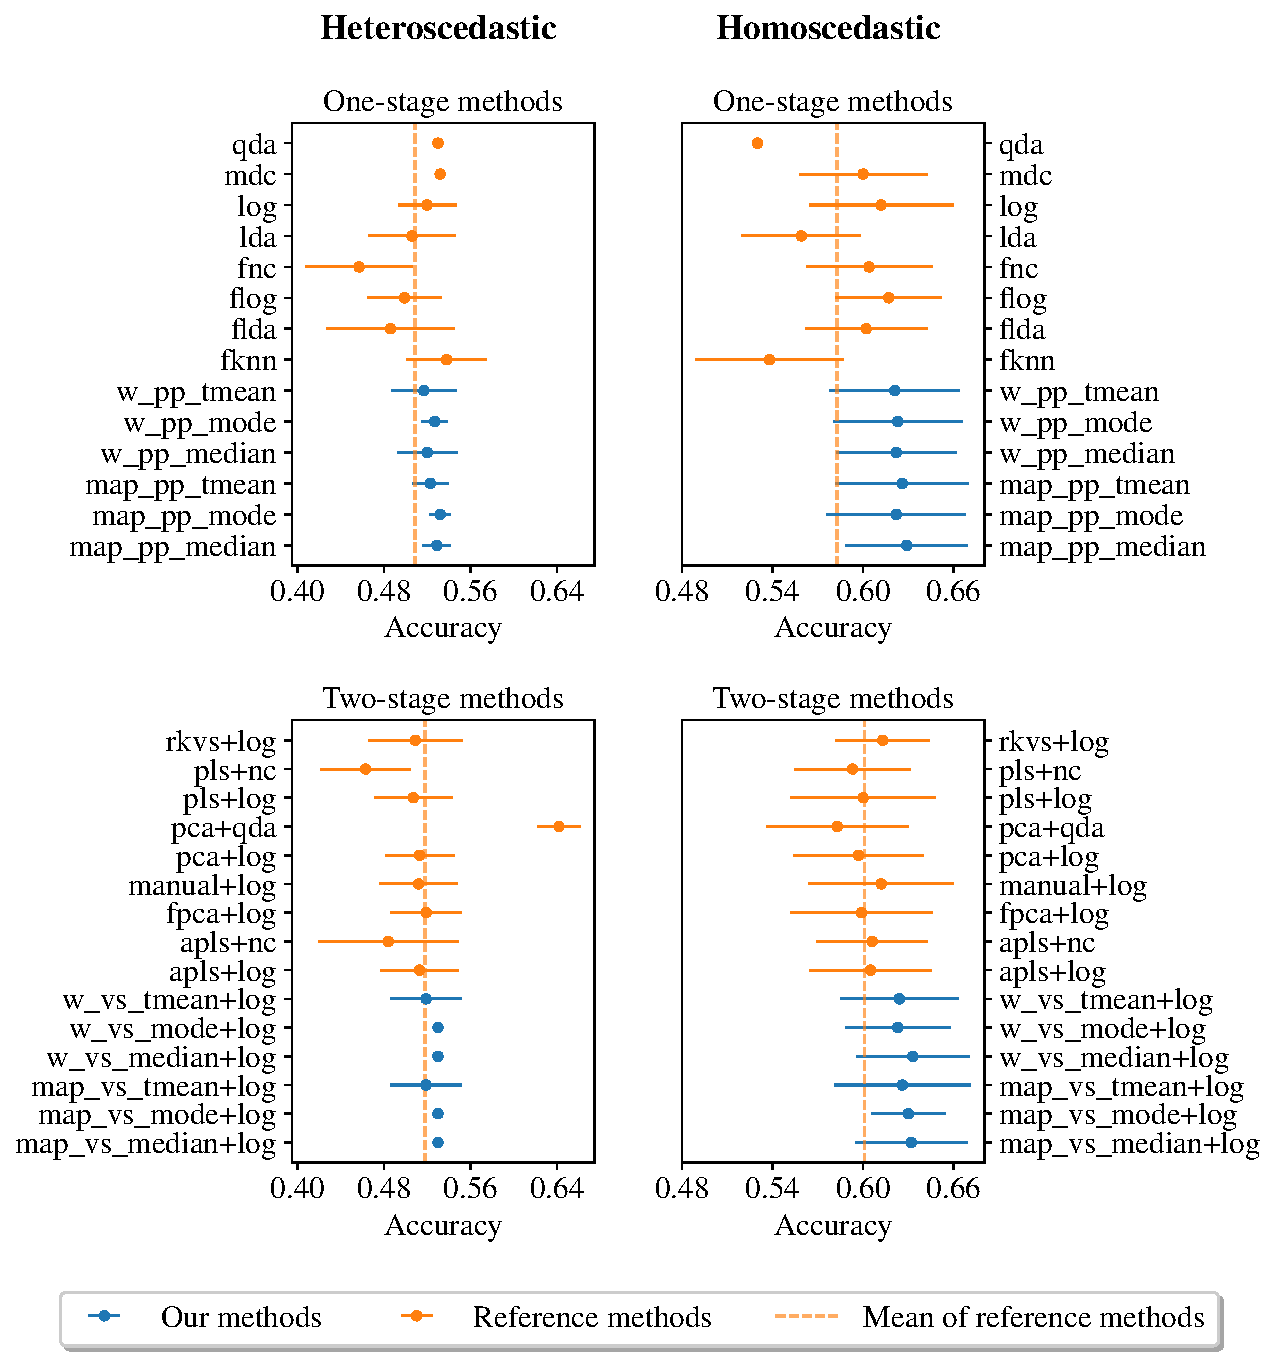
\includegraphics[width=.6\textwidth]{clf_non_gp}
  \caption{Mean and standard error of accuracy of classifiers (higher is better) for 10 runs with a mix of regressors coming from two different GPs and labeled according to their origin. In the first column we try to separate two Brownian motions with the same mean but different variance, while in the second column we discriminate between two Brownian motions with different mean functions but the same variance.}\label{fig:clf_non_gp}
\end{figure}

\subsection{Analysis and validation of a model}\label{app:validation}

We give an example through a series of visual representations of how one would analyze the outcome of our Bayesian methods. This is a preliminary step that comes before prediction; the idea is to validate the model and make sure that the resulting samples from the posterior are coherent and useful. For this illustration we consider a data set used in the experiments, for example the one with squared exponential GP regressors and an underlying linear RKHS response given by
\[
Y=5 - 5X(0.1) + 5X(0.6) + 10X(0.8) + \varepsilon, 
\] 
with \(\varepsilon \sim \mathcal N(0, 0.5)\) (see Figure~\ref{fig:dataset-linear}). We run the sampler for \(3000\) iterations and discard the first \(2000\), with a \(\text{Poisson}(3)\) prior truncated to \(\{1,\dots,5\}\) for \(p\).

\begin{figure}[ht!]
  \centering
  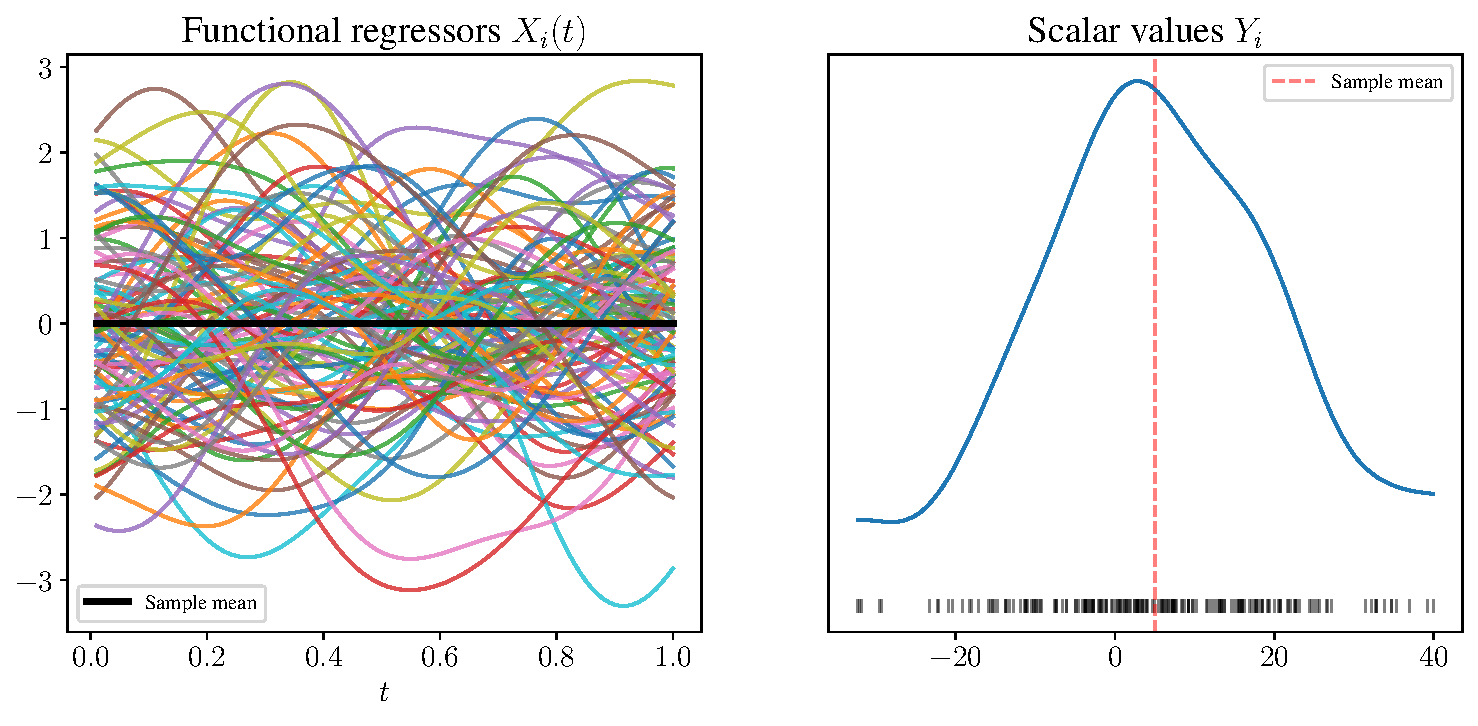
\includegraphics[width=.7\textwidth]{reg_analysis_dataset}
  \caption{Data set with squared exponential GP regressors and linear RKHS response.}\label{fig:dataset-linear}
\end{figure}

The first thing we do is look at arbitrary samples in the last iteration of a few chains, to check that we get reasonable values. Then, we examine the acceptance rate of all the moves to see that they are not either very low or very high. Lastly, we compute the so-called Gelman-Rubin statistic \citep{gelman1992inference}, which is a quantitative measurement of the convergence of the chains (it should be near \(1\)).

Next we proceed with the visual checks. We can look at the flat posterior distribution of all parameters for all values of \(p\) and all the chains aggregated together (Figure~\ref{fig:flat-posterior-linear}), or visualize the posterior of the multidimensional parameters for each \(p\) in a sort of triangular configuration (Figure~\ref{fig:triangular-posterior-linear}). In addition, we can also look at the traces of individual parameters for all values of \(p\) (Figure~\ref{fig:trace-plot}).

\begin{figure}[ht!]
  \centering
  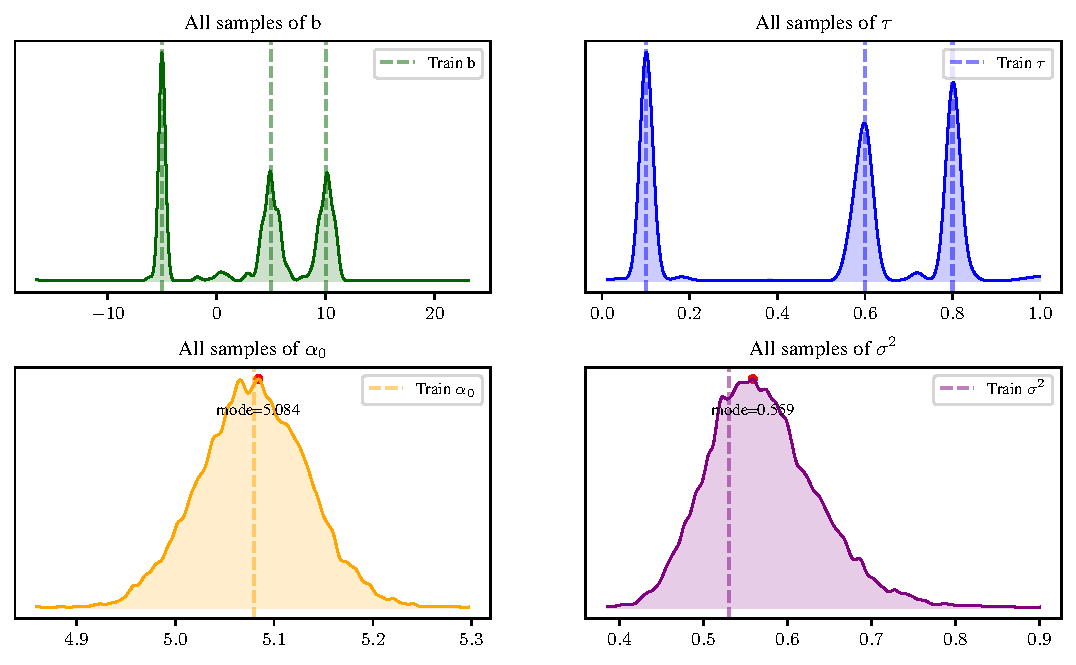
\includegraphics[width=.7\textwidth]{reg_analysis_flat_posterior}
  \caption{Aggregated posterior distribution of all the samples \(\theta^*_{p_m}\) for all \(m\). Note that the true values of the parameters are essentially recovered.}\label{fig:flat-posterior-linear}
\end{figure}

\begin{figure}[ht!]
  \centering
  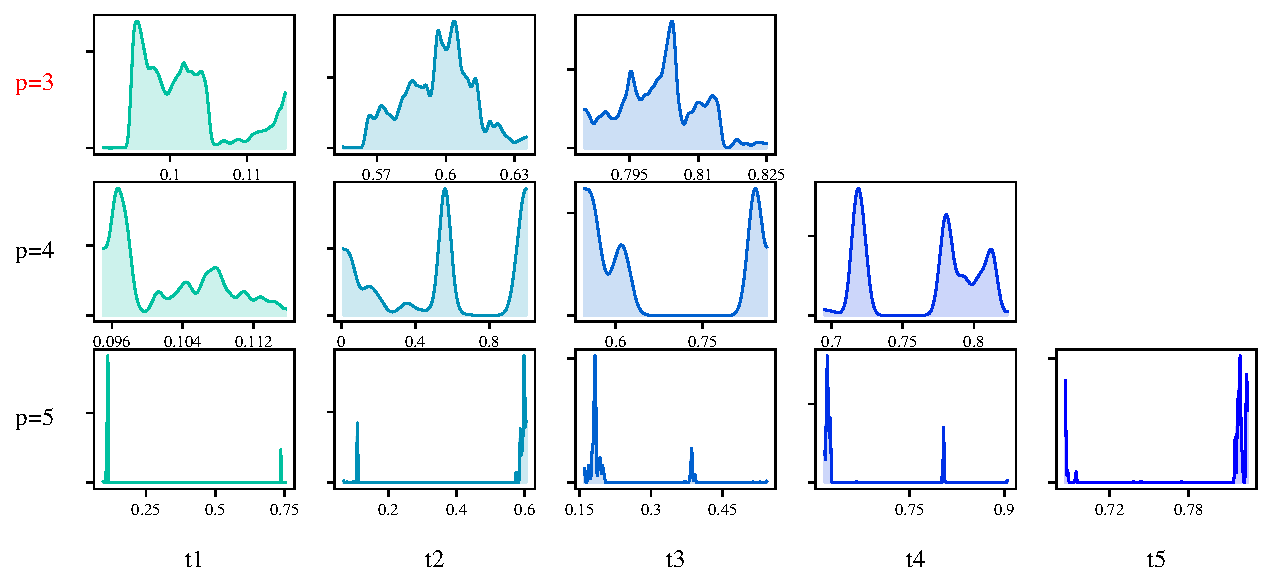
\includegraphics[width=.7\textwidth]{reg_analysis_triangular_posterior}
  \caption{Posterior distribution of \(\tau_p^*\) for each \(p\). The most frequent value is \(p=3\), highlighted in red. In this run there were no samples with \(p=1\) or \(p=2\) after burn-in.}\label{fig:triangular-posterior-linear}
  \end{figure}
  
  \begin{figure}[ht!]
  \centering
  \begin{subfigure}[b]{.75\textwidth}
    \centering
    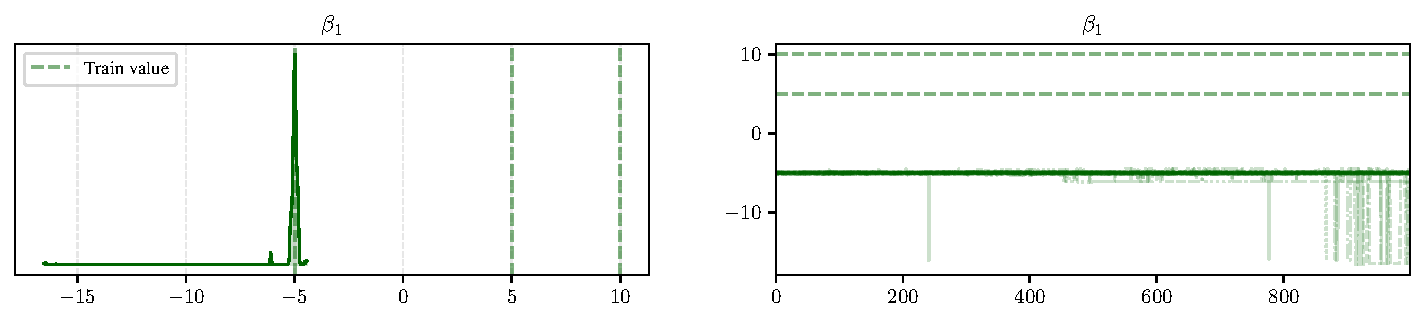
\includegraphics[width=\textwidth]{reg_analysis_trace_1}
  \end{subfigure}
  \begin{subfigure}[b]{.75\textwidth}
    \centering
    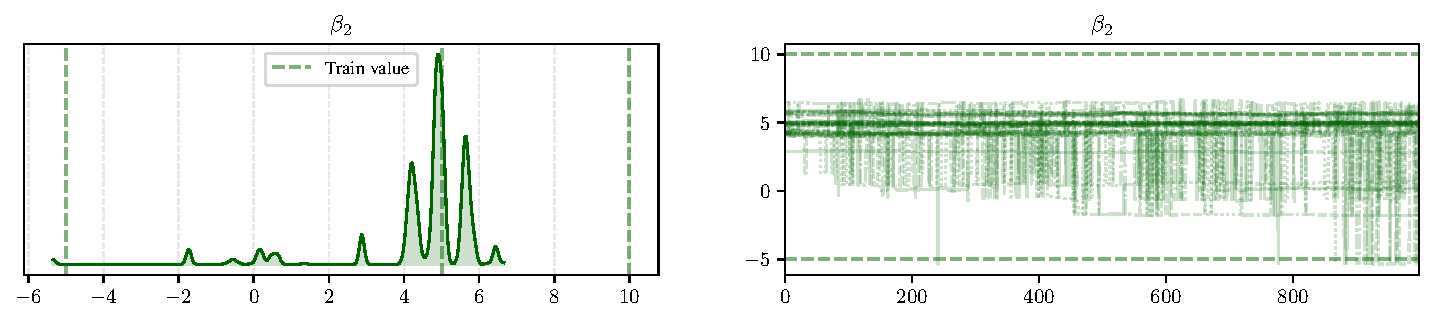
\includegraphics[width=\textwidth]{reg_analysis_trace_2}
  \end{subfigure}
  \begin{subfigure}[b]{.75\textwidth}
      \centering
      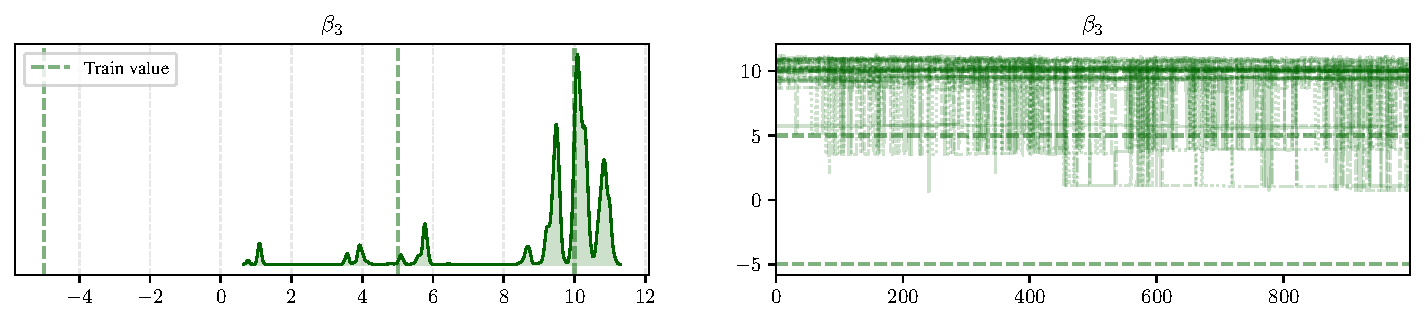
\includegraphics[width=\textwidth]{reg_analysis_trace_3}
  \end{subfigure}
  \begin{subfigure}[b]{.75\textwidth}
      \centering
      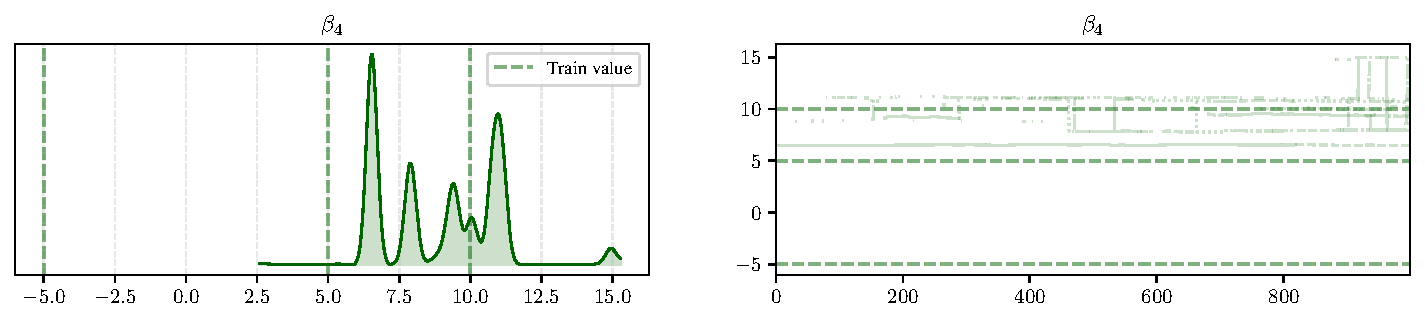
\includegraphics[width=\textwidth]{reg_analysis_trace_4}
  \end{subfigure}
  \begin{subfigure}[b]{.75\textwidth}
      \centering
      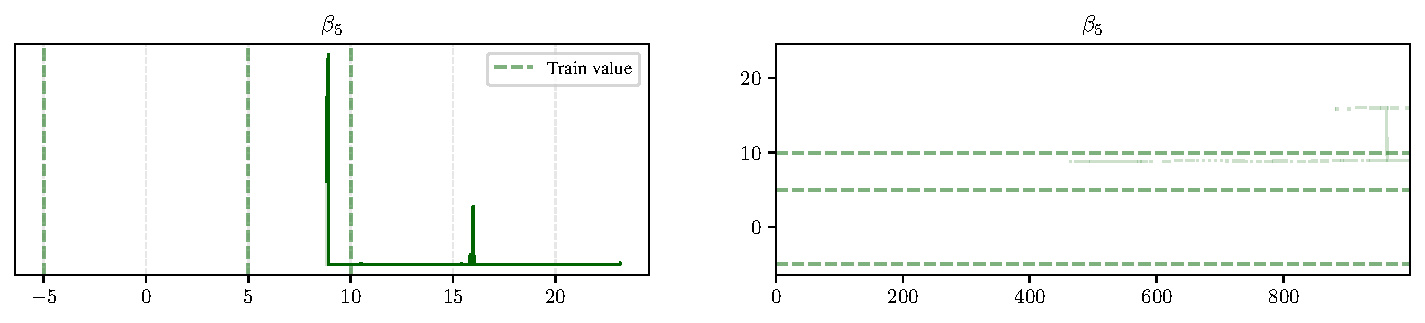
\includegraphics[width=\textwidth]{reg_analysis_trace_5}
  \end{subfigure}
  \caption{Posterior distribution (left) and trace (right) of all the \(\beta_j^*\), combined for all \(p\).}\label{fig:trace-plot}
\end{figure}

\FloatBarrier{}

Looking at the traces is useful to check that the chains are mixing well and that they are correctly exploring the parameter space. We can do the same thing with the values of \(p\) (Figure~\ref{fig:trace-p}). Moreover, we can visualize the tempered posterior distribution of \(p\), that is, the posterior distribution of \(p\) for each temperature (Figure~\ref{fig:tempered-posterior-p}).

\begin{figure}[ht!]
  \centering
  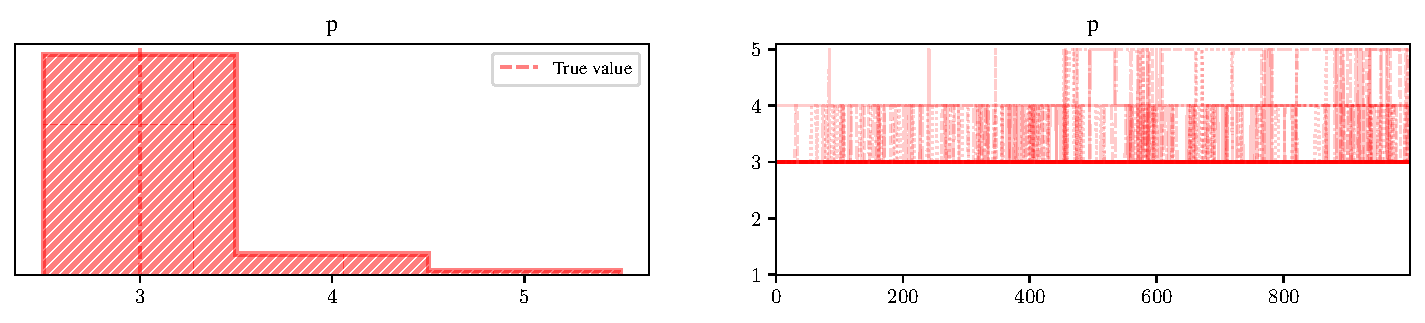
\includegraphics[width=.85\textwidth]{reg_analysis_trace_p}
  \caption{Posterior distribution (left) and trace (right) of \(p\). We see that the true number of components is recovered.}\label{fig:trace-p}
\end{figure}

\begin{figure}[ht!]
  \centering
  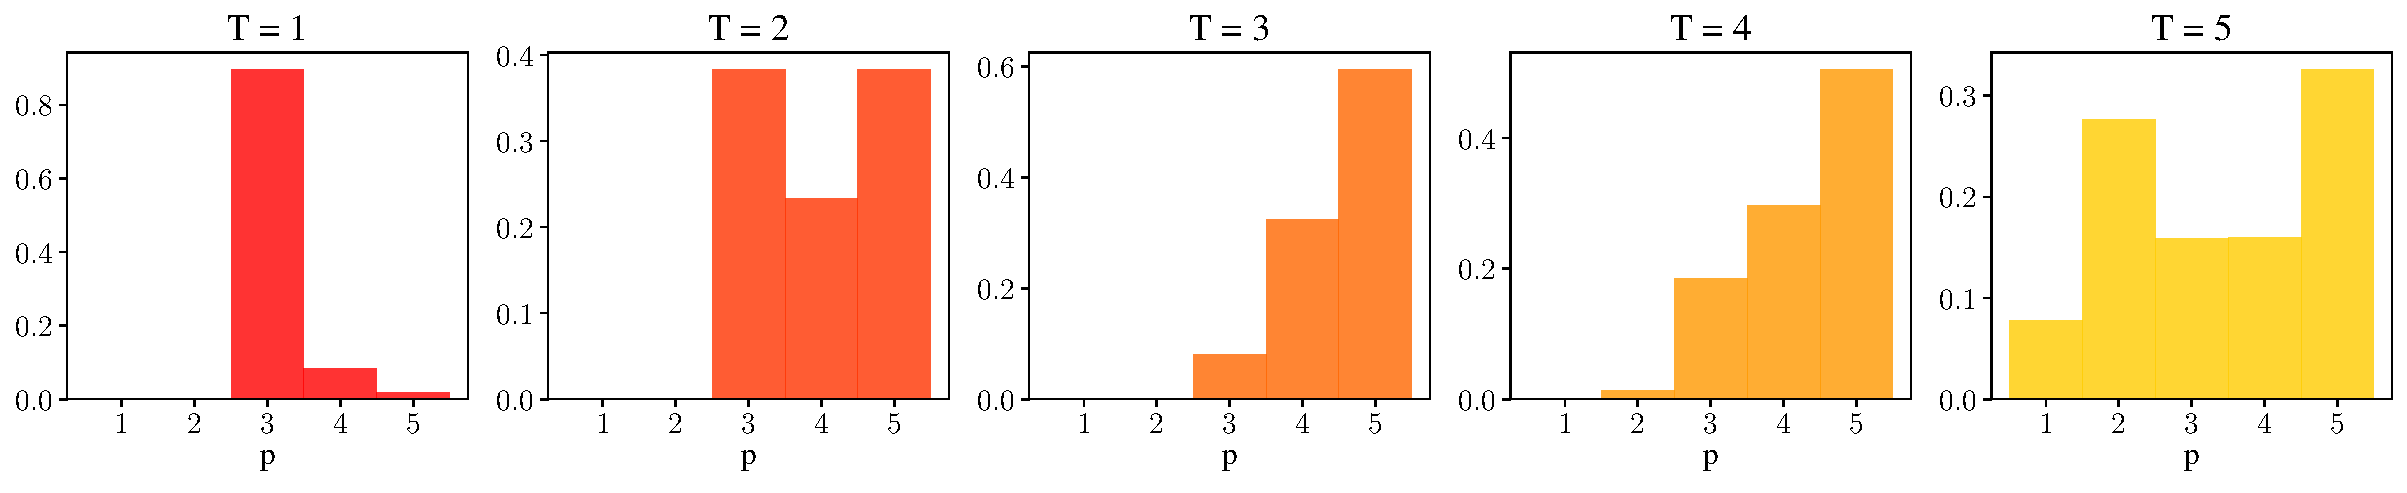
\includegraphics[width=.85\textwidth]{reg_analysis_tempered_posterior_p}
  \caption{Tempered posterior distribution of \(p\). We are only interested in the cold chain (\(T=1\)), but by allowing different temperatures we increase the exploration of the parameter space, periodically transferring some of this information to the cold chain.}\label{fig:tempered-posterior-p}
\end{figure}

Lastly, we can perform a posterior predictive check (Figure~\ref{fig:pp-check}). This is arguably the most useful test for prediction purposes, since we represent the posterior predictive distribution that will be used for inference and prediction. We can do it on the training data or directly on previously unseen regressors. If the sampling has been successful, the posterior predictive should look like a tubular region around the observed data.

\enlargethispage{4\baselineskip}
\begin{figure}[ht!]
  \centering
  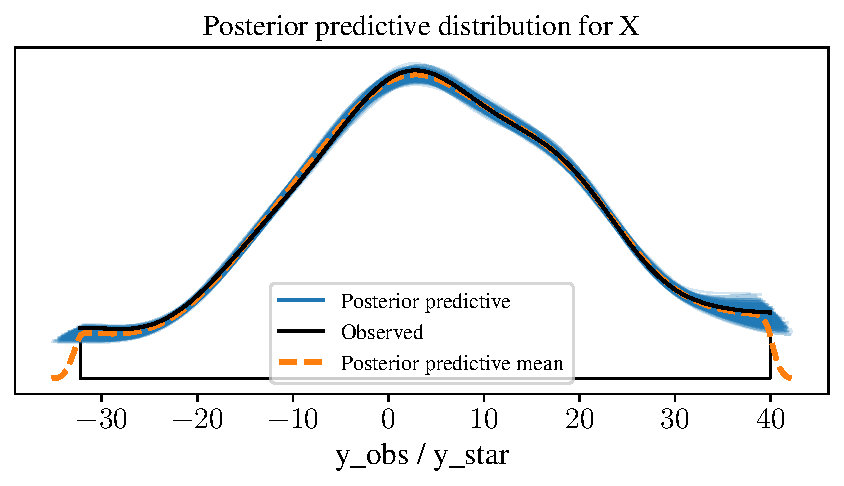
\includegraphics[width=.7\textwidth]{reg_analysis_pp_check}
  \caption{Posterior predictive distribution \(Y|X, \theta_{p_m}^*\) for each individual chain \(m\), along with the mean of all chains and the actual observed data \(Y\).}\label{fig:pp-check}
\end{figure}

\FloatBarrier{}

\subsection{Execution times}\label{app:execution-times}

In Figure~\ref{fig:reg-execution-times} and Figure~\ref{fig:clf-execution-times} we show the execution times of all the experiments in Appendix~\ref{app:non-gp} and Section~\ref{sec:results}. 

\begin{figure}[ht!]
  \centering
  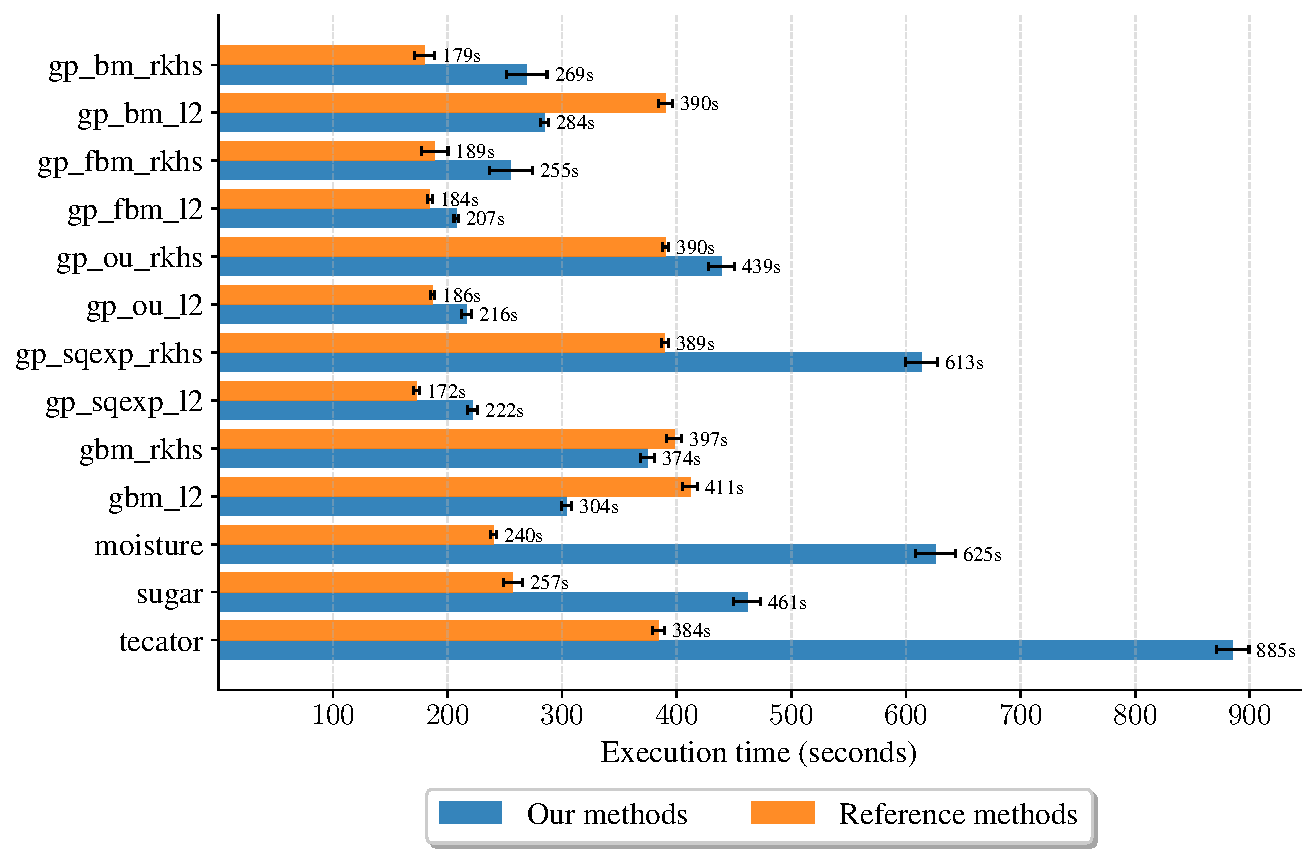
\includegraphics[width=.75\textwidth]{reg_execution_times}
  \caption{Mean and standard error of execution times for all splits in the experiments with the functional linear model.}\label{fig:reg-execution-times}
\end{figure}

\begin{figure}[ht!]
  \centering
  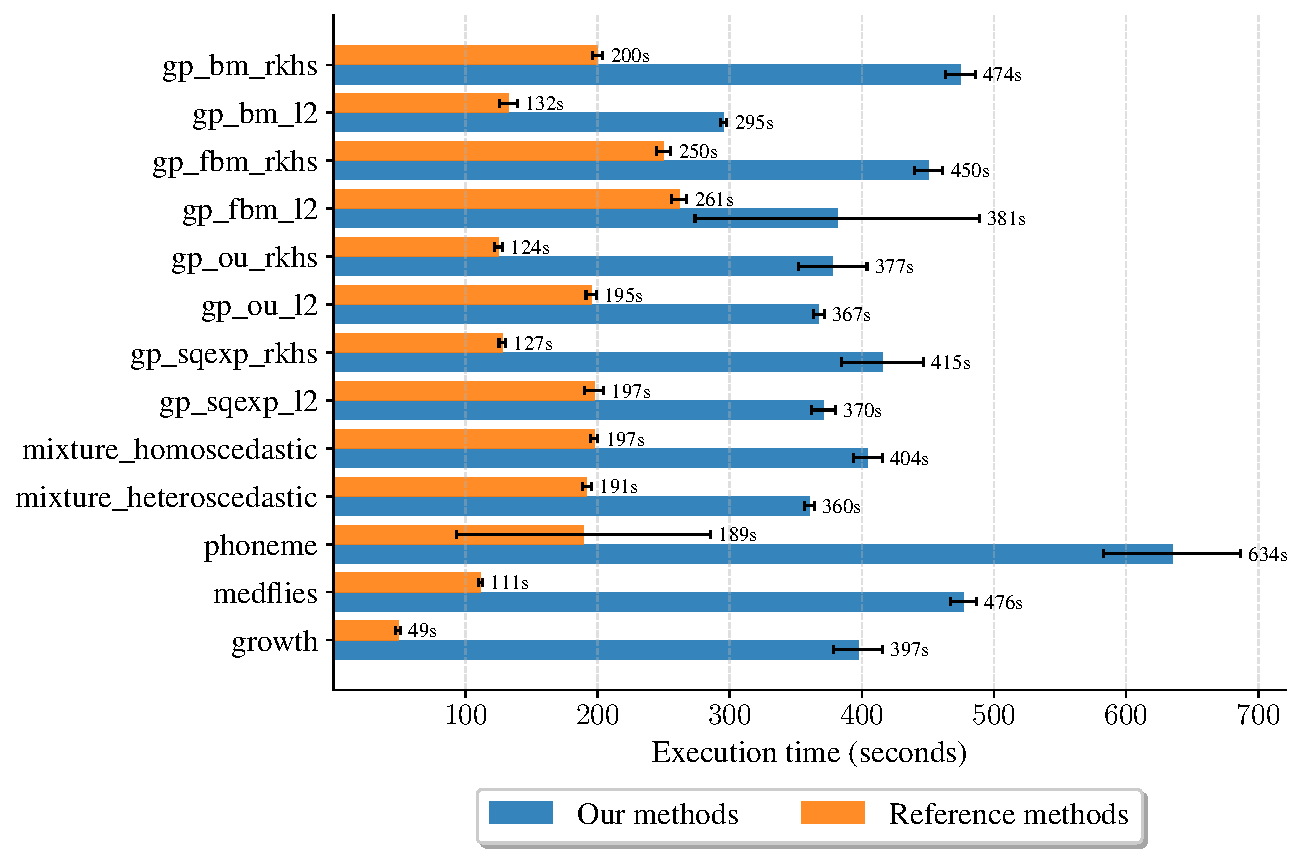
\includegraphics[width=.75\textwidth]{clf_execution_times}
  \caption{Mean and standard error of execution times for all splits in the experiments with the functional logistic model.}\label{fig:clf-execution-times}
\end{figure}

The execution times of the reference methods includes the duration of the cross-validation phase to select the best hyperparameters, a phase that our Bayesian methods lack by design. It is widely known that MCMC sampling tends to be slow, but as we can see the differences are manageable and our methods have reasonable run times for practical use, especially when taking into account the predictive improvement obtained in some cases. 

In addition, it is possible that we ran some MCMC chains for more steps than necessary, because we wanted to perform all experiments in the same generic configuration. In real-world scenarios one would pay closer attention to convergence metrics and try to stop the sampling earlier. Moreover, some splits may be artificially long because of the queue system in the cluster used to run the experiments in parallel.


\subsection{Tables of experimental results}\label{app:tables}

Here we present the tables corresponding to the empirical comparison studies in Appendix~\ref{app:non-gp} and Section~\ref{sec:results}, which show the numerical values that were depicted there graphically. In each case the best and second-best results are shown in \firstcolor{bold} and \secondcolor{italicized blue}, respectively.


\newpage
\subsubsection*{Functional linear regression}

\begin{table}[htbp!]
  \footnotesize
  \centering
  \rowcolors{2}{}{teal!8}
  \begin{tabular}{lcccc}
    \toprule
    \textbf{Prediction method} & \textbf{BM}                 & \textbf{fBM}                & \textbf{O-U}                & \textbf{Gaussian}           \\
    \midrule
    pls1 & 0.997 (0.051) & 0.730 (0.042) & 1.065 (0.055) & 0.673 (0.045) \\
    lasso & 0.680 (0.044) & 0.688 (0.031) & 0.684 (0.031) & 0.671 (0.042) \\
    fpls1 & 1.607 (0.078) & 0.751 (0.040) & 2.088 (0.099) & 0.670 (0.046) \\
    flin & 1.829 (0.073) & 0.869 (0.037) & 2.388 (0.078) & 0.957 (0.044) \\
    apls & 0.875 (0.053) & 0.704 (0.044) & 1.005 (0.050) & 0.672 (0.045) \\
    w\_pp\_tmean & \firstcolor{0.668 (0.043)} & \firstcolor{0.676 (0.032)} & 0.676 (0.042) & \firstcolor{0.662 (0.040)} \\
    w\_pp\_mode & 0.670 (0.041) & \firstcolor{0.676 (0.030)} & 0.675 (0.041) & \secondcolor{0.664 (0.040)} \\
    w\_pp\_median & \firstcolor{0.668 (0.043)} & \firstcolor{0.676 (0.032)} & 0.676 (0.042) & \firstcolor{0.662 (0.040)} \\
    map\_pp\_tmean & \secondcolor{0.669 (0.042)} & \secondcolor{0.677 (0.031)} & \secondcolor{0.671 (0.045)} & 0.666 (0.039) \\
    map\_pp\_mode & 0.672 (0.041) & 0.680 (0.029) & 0.672 (0.045) & 0.670 (0.042) \\
    map\_pp\_median & 0.670 (0.043) & \secondcolor{0.677 (0.031)} & \firstcolor{0.670 (0.045)} & 0.667 (0.040) \\
    \bottomrule
    \toprule
    pls+r & 0.996 (0.056) & 0.720 (0.036) & 1.065 (0.055) & 0.674 (0.044) \\
    pca+r & 1.521 (0.070) & 0.720 (0.034) & 2.249 (0.095) & 0.673 (0.045) \\
    manual+r & 1.342 (0.130) & 0.717 (0.040) & 1.719 (0.101) & 0.674 (0.042) \\
    fpls+r & 1.607 (0.078) & 0.752 (0.039) & 2.089 (0.098) & \secondcolor{0.669 (0.046)} \\
    fpca+r & 1.512 (0.071) & 0.721 (0.034) & 2.237 (0.096) & 0.673 (0.045) \\
    w\_vs\_tmean+r & \secondcolor{0.795 (0.069)} & 0.697 (0.029) & 0.987 (0.131) & 0.672 (0.037) \\
    w\_vs\_mode+r & \firstcolor{0.668 (0.040)} & \firstcolor{0.678 (0.034)} & 0.667 (0.041) & 0.680 (0.050) \\
    w\_vs\_median+r & \firstcolor{0.668 (0.039)} & 0.681 (0.031) & \secondcolor{0.666 (0.041)} & \firstcolor{0.666 (0.041)} \\
    map\_vs\_tmean+r & \firstcolor{0.668 (0.040)} & 0.747 (0.048) & 0.971 (0.398) & 0.737 (0.093) \\
    map\_vs\_mode+r & \firstcolor{0.668 (0.040)} & \secondcolor{0.679 (0.034)} & 0.668 (0.042) & 0.707 (0.037) \\
    map\_vs\_median+r & \firstcolor{0.668 (0.040)} & 0.695 (0.029) & \firstcolor{0.664 (0.041)} & 0.700 (0.063) \\
    \bottomrule
  \end{tabular}
  \caption{Mean RMSE of predictors (lower is better) for 10 runs with GP regressors, one on each column, that obey an underlying linear RKHS model. The corresponding standard errors are shown between brackets.}
\end{table}
\FloatBarrier{}
\newpage


\begin{table}[htbp!]
  \vspace{1em}
  \footnotesize
  \centering
  \rowcolors{2}{}{teal!8}
  \begin{tabular}{lcccc}
    \toprule
    \textbf{Prediction method} & \textbf{BM}                 & \textbf{fBM}                & \textbf{O-U}                & \textbf{Gaussian}           \\
    \midrule
    pls1 & 0.678 (0.039) & 0.674 (0.030) & 0.682 (0.043) & 0.669 (0.047) \\
    lasso & 0.667 (0.037) & 0.664 (0.035) & 0.659 (0.039) & 0.664 (0.041) \\
    fpls1 & 0.671 (0.041) & 0.671 (0.044) & 0.677 (0.037) & 0.671 (0.048) \\
    flin & 0.666 (0.037) & 0.664 (0.038) & 0.662 (0.038) & \firstcolor{0.661 (0.040)} \\
    apls & 0.673 (0.045) & 0.684 (0.043) & 0.681 (0.043) & 0.674 (0.041) \\
    w\_pp\_tmean & \firstcolor{0.652 (0.037)} & \firstcolor{0.659 (0.039)} & \firstcolor{0.651 (0.037)} & \firstcolor{0.661 (0.039)} \\
    w\_pp\_mode & 0.655 (0.037) & \secondcolor{0.661 (0.038)} & \secondcolor{0.652 (0.037)} & \firstcolor{0.661 (0.039)} \\
    w\_pp\_median & \firstcolor{0.652 (0.037)} & \firstcolor{0.659 (0.039)} & \firstcolor{0.651 (0.037)} & \firstcolor{0.661 (0.039)} \\
    map\_pp\_tmean & \secondcolor{0.654 (0.037)} & \secondcolor{0.661 (0.038)} & 0.655 (0.038) & \firstcolor{0.661 (0.039)} \\
    map\_pp\_mode & 0.655 (0.035) & 0.664 (0.039) & 0.656 (0.037) & \secondcolor{0.662 (0.037)} \\
    map\_pp\_median & \secondcolor{0.654 (0.037)} & \secondcolor{0.661 (0.038)} & 0.655 (0.038) & \firstcolor{0.661 (0.039)} \\
    \bottomrule
    \toprule
    pls+r & 0.667 (0.037) & 0.669 (0.033) & 0.669 (0.037) & \firstcolor{0.665 (0.044)} \\
    pca+r & 0.665 (0.041) & 0.664 (0.041) & 0.665 (0.041) & \secondcolor{0.666 (0.044)} \\
    manual+r & 0.665 (0.035) & \firstcolor{0.660 (0.037)} & 0.664 (0.040) & \secondcolor{0.666 (0.046)} \\
    fpls+r & 0.666 (0.040) & 0.664 (0.042) & 0.672 (0.036) & 0.668 (0.047) \\
    fpca+r & 0.665 (0.042) & 0.665 (0.042) & 0.663 (0.040) & \secondcolor{0.666 (0.045)} \\
    w\_vs\_tmean+r & \firstcolor{0.651 (0.038)} & \firstcolor{0.660 (0.039)} & \firstcolor{0.649 (0.036)} & 0.675 (0.039) \\
    w\_vs\_mode+r & 0.660 (0.037) & 0.662 (0.039) & 0.663 (0.032) & 0.673 (0.046) \\
    w\_vs\_median+r & \secondcolor{0.652 (0.036)} & \firstcolor{0.660 (0.038)} & \secondcolor{0.653 (0.039)} & 0.672 (0.039) \\
    map\_vs\_tmean+r & 0.654 (0.037) & \secondcolor{0.661 (0.037)} & 0.659 (0.039) & 0.674 (0.041) \\
    map\_vs\_mode+r & 0.661 (0.036) & 0.667 (0.040) & 0.670 (0.036) & 0.704 (0.058) \\
    map\_vs\_median+r & 0.655 (0.035) & 0.663 (0.035) & 0.662 (0.043) & 0.678 (0.042) \\
    \bottomrule
  \end{tabular}
  \caption{Mean RMSE of predictors (lower is better) for 10 runs with GP regressors, one on each column, that obey an underlying linear \(L^2\)-model. The corresponding standard errors are shown between brackets.}
\end{table}
\newpage
\FloatBarrier{}

\begin{table}[htbp!]
  \vspace{1em}
  \footnotesize
  \centering
  \rowcolors{2}{}{teal!8}
  \begin{tabular}{lcc}
    \toprule
    \textbf{Prediction method} & \textbf{GBM + \(\bf{L^2}\)} & \textbf{GBM + RKHS}         \\
    \midrule
    pls1 & 0.668 (0.034) & 1.579 (0.145) \\
    lasso & \secondcolor{0.657 (0.041)} & 0.676 (0.046) \\
    fpls1 & 0.666 (0.035) & 2.654 (0.182) \\
    flin & 0.660 (0.037) & 3.434 (0.384) \\
    apls & 0.662 (0.040) & 1.100 (0.100) \\
    w\_pp\_tmean & \firstcolor{0.655 (0.042)} & \firstcolor{0.662 (0.039)} \\
    w\_pp\_mode & 0.659 (0.043) & 0.666 (0.036) \\
    w\_pp\_median & \firstcolor{0.655 (0.042)} & \firstcolor{0.662 (0.039)} \\
    map\_pp\_tmean & \secondcolor{0.657 (0.043)} & \secondcolor{0.665 (0.038)} \\
    map\_pp\_mode & 0.659 (0.041) & 0.670 (0.037) \\
    map\_pp\_median & \secondcolor{0.657 (0.043)} & \secondcolor{0.665 (0.038)} \\
    \bottomrule
    \toprule
    pls+r & 0.661 (0.040) & 1.574 (0.141) \\
    pca+r & 0.658 (0.040) & 2.315 (0.195) \\
    manual+r & 0.665 (0.039) & 1.478 (0.154) \\
    fpls+r & 0.665 (0.037) & 2.669 (0.189) \\
    fpca+r & 0.659 (0.040) & 2.311 (0.194) \\
    w\_vs\_tmean+r & \firstcolor{0.655 (0.040)} & 0.986 (0.186) \\
    w\_vs\_mode+r & 0.661 (0.044) & \secondcolor{0.665 (0.038)} \\
    w\_vs\_median+r & \secondcolor{0.656 (0.042)} & \firstcolor{0.663 (0.037)} \\
    map\_vs\_tmean+r & 0.662 (0.042) & \secondcolor{0.665 (0.038)} \\
    map\_vs\_mode+r & 0.669 (0.044) & \secondcolor{0.665 (0.038)} \\
    map\_vs\_median+r & 0.663 (0.044) & \secondcolor{0.665 (0.038)} \\
    \bottomrule
  \end{tabular}
  \caption{Mean RMSE of predictors (lower is better) for 10 runs with GBM regressors. In the first column the response obeys a linear \(L^2\)-model, while in the second column it follows a linear RKHS model. The corresponding standard errors are shown between brackets.}
\end{table}
\newpage
\FloatBarrier{}

\begin{table}[htbp!]
  \vspace{1em}
  \footnotesize
  \centering
  \rowcolors{2}{}{teal!8}
  \begin{tabular}{lccc}
    \toprule
    \textbf{Prediction method} & \textbf{Moisture}           & \textbf{Sugar}              & \textbf{Tecator}            \\
    \midrule
    pls1 & 0.232 (0.024) & 2.037 (0.219) & \secondcolor{2.606 (0.283)} \\
    lasso & 0.242 (0.026) & 1.985 (0.226) & 2.842 (0.352) \\
    fpls1 & 0.248 (0.022) & \secondcolor{1.972 (0.201)} & \firstcolor{2.605 (0.262)} \\
    flin & 1.235 (0.138) & \firstcolor{1.966 (0.198)} & 7.486 (0.648) \\
    apls & 0.237 (0.028) & 2.020 (0.226) & 2.641 (0.165) \\
    w\_pp\_tmean & \secondcolor{0.223 (0.018)} & 1.988 (0.216) & 2.721 (0.260) \\
    w\_pp\_mode & \firstcolor{0.222 (0.020)} & 1.996 (0.219) & 2.718 (0.266) \\
    w\_pp\_median & \secondcolor{0.223 (0.018)} & 1.989 (0.217) & 2.721 (0.262) \\
    map\_pp\_tmean & 0.228 (0.021) & 1.997 (0.212) & 2.724 (0.267) \\
    map\_pp\_mode & 0.236 (0.023) & 2.010 (0.210) & 2.741 (0.271) \\
    map\_pp\_median & 0.228 (0.021) & 1.996 (0.212) & 2.720 (0.267) \\
    \bottomrule
    \toprule
    pls+r & \firstcolor{0.225 (0.021)} & \secondcolor{1.998 (0.208)} & \firstcolor{2.536 (0.236)} \\
    pca+r & \secondcolor{0.233 (0.024)} & 2.034 (0.219) & 2.712 (0.183) \\
    manual+r & 0.268 (0.021) & 2.041 (0.214) & \secondcolor{2.586 (0.270)} \\
    fpls+r & 0.241 (0.018) & \firstcolor{1.962 (0.202)} & 2.595 (0.249) \\
    fpca+r & 0.307 (0.055) & 2.054 (0.226) & 2.657 (0.189) \\
    w\_vs\_tmean+r & 0.308 (0.075) & 2.003 (0.221) & 2.822 (0.323) \\
    w\_vs\_mode+r & 0.236 (0.018) & 2.050 (0.221) & 2.713 (0.255) \\
    w\_vs\_median+r & 0.236 (0.025) & 2.000 (0.217) & 2.801 (0.261) \\
    map\_vs\_tmean+r & 0.455 (0.284) & 2.059 (0.233) & 2.900 (0.403) \\
    map\_vs\_mode+r & 0.261 (0.029) & 2.188 (0.321) & 2.833 (0.291) \\
    map\_vs\_median+r & 0.266 (0.030) & 2.082 (0.219) & 2.826 (0.269) \\
    \bottomrule
  \end{tabular}
  \caption{Mean RMSE of predictors (lower is better) for 10 runs with real data sets, one on each column. The corresponding standard errors are shown between brackets.}
\end{table}
\newpage
\FloatBarrier{}

\subsubsection*{Functional logistic regression}

\begin{table}[htbp!]
  \footnotesize
  \centering
  \rowcolors{2}{}{teal!8}
  \begin{tabular}{lcccc}
    \toprule
    \textbf{Classification method} & \textbf{BM}                 & \textbf{fBM}                & \textbf{O-U}                & \textbf{Gaussian}           \\
    \midrule
    qda & 0.510 (0.000) & 0.510 (0.000) & 0.510 (0.000) & 0.500 (0.000) \\
    mdc & 0.804 (0.034) & 0.822 (0.022) & 0.735 (0.037) & 0.839 (0.045) \\
    log & 0.849 (0.031) & \firstcolor{0.848 (0.015)} & 0.824 (0.022) & 0.868 (0.036) \\
    lda & 0.694 (0.032) & 0.621 (0.066) & 0.624 (0.042) & 0.823 (0.028) \\
    fnc & 0.814 (0.034) & \firstcolor{0.848 (0.014)} & 0.736 (0.035) & 0.864 (0.046) \\
    flog & 0.845 (0.036) & 0.837 (0.024) & 0.809 (0.028) & 0.871 (0.033) \\
    flda & 0.846 (0.031) & 0.830 (0.029) & 0.813 (0.029) & 0.854 (0.039) \\
    fknn & 0.851 (0.033) & 0.834 (0.027) & 0.799 (0.024) & 0.847 (0.041) \\
    w\_pp\_tmean & \firstcolor{0.856 (0.030)} & 0.846 (0.011) & 0.828 (0.022) & 0.873 (0.035) \\
    w\_pp\_mode & 0.853 (0.031) & \secondcolor{0.847 (0.012)} & 0.825 (0.025) & \firstcolor{0.878 (0.036)} \\
    w\_pp\_median & \firstcolor{0.856 (0.029)} & \secondcolor{0.847 (0.011)} & 0.827 (0.022) & 0.873 (0.035) \\
    map\_pp\_tmean & 0.854 (0.034) & 0.845 (0.013) & \firstcolor{0.830 (0.025)} & 0.874 (0.035) \\
    map\_pp\_mode & 0.852 (0.032) & 0.846 (0.014) & \secondcolor{0.829 (0.025)} & \secondcolor{0.877 (0.036)} \\
    map\_pp\_median & \secondcolor{0.855 (0.030)} & 0.844 (0.013) & \firstcolor{0.830 (0.025)} & 0.876 (0.036) \\
    \bottomrule
    \toprule
    rkvs+log & \firstcolor{0.848 (0.024)} & 0.838 (0.026) & 0.790 (0.032) & 0.872 (0.041) \\
    pls+nc & 0.816 (0.038) & 0.828 (0.022) & 0.793 (0.029) & 0.867 (0.039) \\
    pls+log & \secondcolor{0.847 (0.034)} & 0.844 (0.021) & 0.817 (0.022) & 0.864 (0.037) \\
    pca+qda & 0.839 (0.034) & 0.840 (0.018) & 0.818 (0.026) & 0.854 (0.033) \\
    pca+log & 0.842 (0.032) & \secondcolor{0.847 (0.016)} & 0.824 (0.019) & 0.868 (0.033) \\
    manual+log & 0.846 (0.032) & \firstcolor{0.850 (0.012)} & 0.821 (0.018) & 0.869 (0.032) \\
    fpca+log & \secondcolor{0.847 (0.030)} & \secondcolor{0.847 (0.014)} & \secondcolor{0.830 (0.024)} & 0.866 (0.036) \\
    apls+nc & 0.819 (0.036) & \secondcolor{0.847 (0.014)} & 0.816 (0.027) & 0.854 (0.036) \\
    apls+log & 0.829 (0.041) & 0.844 (0.012) & 0.816 (0.027) & 0.857 (0.039) \\
    w\_vs\_tmean+log & 0.831 (0.038) & 0.840 (0.017) & 0.823 (0.033) & 0.873 (0.038) \\
    w\_vs\_mode+log & 0.846 (0.021) & 0.828 (0.019) & 0.806 (0.020) & 0.875 (0.040) \\
    w\_vs\_median+log & 0.838 (0.029) & 0.844 (0.017) & \firstcolor{0.834 (0.030)} & 0.875 (0.039) \\
    map\_vs\_tmean+log & 0.816 (0.028) & 0.838 (0.023) & 0.801 (0.027) & \secondcolor{0.876 (0.040)} \\
    map\_vs\_mode+log & 0.839 (0.022) & 0.831 (0.022) & 0.807 (0.014) & \firstcolor{0.877 (0.043)} \\
    map\_vs\_median+log & 0.829 (0.024) & 0.839 (0.019) & 0.816 (0.034) & 0.871 (0.048) \\
    \bottomrule
  \end{tabular}
  \caption{Mean accuracy of classifiers (higher is better) for 10 runs with GP regressors, one on each column, that obey an underlying logistic RKHS model. The corresponding standard errors are shown between brackets.}
\end{table}
\newpage
\FloatBarrier{}

\begin{table}[htbp!]
  \vspace{1em}
  \footnotesize
  \centering
  \rowcolors{2}{}{teal!8}
  \begin{tabular}{lcccc}
    \toprule
    \textbf{Classification method} & \textbf{BM}                 & \textbf{fBM}                & \textbf{O-U}                & \textbf{Gaussian}           \\
    \midrule
    qda & \firstcolor{0.610 (0.000)} & 0.610 (0.000) & \firstcolor{0.620 (0.000)} & \secondcolor{0.610 (0.000)} \\
    mdc & 0.602 (0.033) & \firstcolor{0.619 (0.048)} & \secondcolor{0.615 (0.029)} & 0.603 (0.042) \\
    log & 0.594 (0.017) & 0.577 (0.039) & 0.591 (0.024) & 0.609 (0.037) \\
    lda & 0.507 (0.030) & 0.518 (0.029) & 0.541 (0.039) & 0.591 (0.033) \\
    fnc & \secondcolor{0.607 (0.038)} & \secondcolor{0.614 (0.045)} & 0.609 (0.029) & \firstcolor{0.625 (0.040)} \\
    flog & 0.580 (0.020) & 0.602 (0.037) & 0.600 (0.031) & 0.609 (0.028) \\
    flda & 0.601 (0.027) & 0.609 (0.049) & 0.593 (0.032) & 0.595 (0.048) \\
    fknn & 0.587 (0.056) & 0.576 (0.033) & 0.564 (0.042) & 0.578 (0.041) \\
    w\_pp\_tmean & 0.597 (0.027) & 0.600 (0.026) & 0.592 (0.023) & 0.608 (0.035) \\
    w\_pp\_mode & 0.599 (0.028) & 0.606 (0.027) & 0.595 (0.030) & 0.605 (0.034) \\
    w\_pp\_median & 0.597 (0.023) & 0.599 (0.030) & 0.591 (0.020) & 0.607 (0.037) \\
    map\_pp\_tmean & 0.595 (0.022) & 0.599 (0.027) & 0.594 (0.020) & 0.602 (0.037) \\
    map\_pp\_mode & 0.605 (0.027) & 0.604 (0.030) & 0.602 (0.030) & 0.606 (0.041) \\
    map\_pp\_median & 0.593 (0.026) & 0.599 (0.028) & 0.600 (0.023) & 0.602 (0.034) \\
    \bottomrule
    \toprule
    rkvs+log & 0.569 (0.039) & 0.586 (0.026) & 0.593 (0.035) & 0.611 (0.034) \\
    pls+nc & \firstcolor{0.610 (0.033)} & \firstcolor{0.623 (0.042)} & \firstcolor{0.607 (0.035)} & \firstcolor{0.629 (0.036)} \\
    pls+log & 0.590 (0.029) & 0.589 (0.036) & 0.593 (0.020) & \secondcolor{0.621 (0.043)} \\
    pca+qda & 0.577 (0.036) & \secondcolor{0.615 (0.032)} & 0.599 (0.043) & 0.618 (0.045) \\
    pca+log & 0.590 (0.027) & 0.593 (0.027) & 0.598 (0.037) & 0.616 (0.036) \\
    manual+log & 0.580 (0.026) & 0.585 (0.030) & 0.593 (0.019) & \secondcolor{0.621 (0.044)} \\
    fpca+log & \secondcolor{0.599 (0.021)} & 0.592 (0.034) & 0.600 (0.039) & 0.614 (0.042) \\
    apls+nc & 0.593 (0.024) & 0.569 (0.047) & 0.591 (0.039) & 0.615 (0.023) \\
    apls+log & 0.571 (0.030) & 0.585 (0.033) & 0.594 (0.025) & 0.614 (0.038) \\
    w\_vs\_tmean+log & 0.588 (0.034) & 0.594 (0.022) & 0.596 (0.017) & 0.605 (0.029) \\
    w\_vs\_mode+log & 0.597 (0.024) & 0.597 (0.028) & \secondcolor{0.601 (0.026)} & 0.617 (0.026) \\
    w\_vs\_median+log & 0.591 (0.030) & 0.589 (0.023) & 0.599 (0.035) & 0.600 (0.031) \\
    map\_vs\_tmean+log & 0.590 (0.031) & 0.594 (0.026) & 0.589 (0.030) & 0.609 (0.031) \\
    map\_vs\_mode+log & 0.597 (0.024) & 0.593 (0.022) & 0.599 (0.027) & 0.617 (0.021) \\
    map\_vs\_median+log & 0.587 (0.036) & 0.592 (0.021) & 0.598 (0.036) & 0.605 (0.034) \\
    \bottomrule
  \end{tabular}
  \caption{Mean accuracy of classifiers (higher is better) for 10 runs with GP regressors, one on each column, that obey an underlying logistic \(L^2\)-model. The corresponding standard errors are shown between brackets.}
\end{table}
\newpage
\FloatBarrier{}

\begin{table}[htbp!]
  \vspace{1em}
  \footnotesize
  \centering
  \rowcolors{2}{}{teal!8}
  \begin{tabular}{lcccc}
    \toprule
    \textbf{Classification method} & \textbf{Heteroscedastic}    & \textbf{Homoscedastic}      \\
    \midrule
    qda & 0.530 (0.000) & 0.530 (0.000) \\
    mdc & \secondcolor{0.532 (0.004)} & 0.600 (0.042) \\
    log & 0.520 (0.027) & 0.612 (0.048) \\
    lda & 0.506 (0.041) & 0.559 (0.040) \\
    fnc & 0.457 (0.049) & 0.604 (0.042) \\
    flog & 0.499 (0.034) & 0.617 (0.035) \\
    flda & 0.486 (0.059) & 0.602 (0.040) \\
    fknn & \firstcolor{0.538 (0.037)} & 0.538 (0.049) \\
    w\_pp\_tmean & 0.517 (0.030) & 0.621 (0.043) \\
    w\_pp\_mode & 0.527 (0.012) & 0.623 (0.043) \\
    w\_pp\_median & 0.520 (0.028) & 0.622 (0.040) \\
    map\_pp\_tmean & 0.523 (0.017) & \secondcolor{0.626 (0.044)} \\
    map\_pp\_mode & \secondcolor{0.532 (0.010)} & 0.622 (0.046) \\
    map\_pp\_median & 0.529 (0.013) & \firstcolor{0.629 (0.040)} \\
    \bottomrule
    \toprule
    rkvs+log & 0.509 (0.044) & 0.613 (0.031) \\
    pls+nc & 0.463 (0.042) & 0.593 (0.038) \\
    pls+log & 0.507 (0.036) & 0.600 (0.048) \\
    pca+qda & \firstcolor{0.642 (0.020)} & 0.583 (0.047) \\
    pca+log & 0.513 (0.032) & 0.597 (0.043) \\
    manual+log & 0.512 (0.036) & 0.612 (0.048) \\
    fpca+log & 0.519 (0.033) & 0.599 (0.047) \\
    apls+nc & 0.484 (0.065) & 0.606 (0.037) \\
    apls+log & 0.513 (0.036) & 0.605 (0.040) \\
    w\_vs\_tmean+log & 0.519 (0.033) & 0.624 (0.039) \\
    w\_vs\_mode+log & \secondcolor{0.530 (0.000)} & 0.623 (0.035) \\
    w\_vs\_median+log & \secondcolor{0.530 (0.000)} & \firstcolor{0.633 (0.037)} \\
    map\_vs\_tmean+log & 0.519 (0.033) & 0.626 (0.045) \\
    map\_vs\_mode+log & \secondcolor{0.530 (0.000)} & 0.630 (0.024) \\
    map\_vs\_median+log & \secondcolor{0.530 (0.000)} & \secondcolor{0.632 (0.037)} \\
    \bottomrule
  \end{tabular}
  \caption{Mean accuracy of classifiers (higher is better) for 10 runs with a mix of regressors coming from two different GPs and labeled according to their origin. In the first column we try to separate two heteroscedastic Brownian motions, while in the second column we discriminate between two homoscedastic Brownian motions. The corresponding standard errors are shown between brackets.}
\end{table}
\newpage
\FloatBarrier{}


\begin{table}[htbp!]
  \vspace{1em}
  \footnotesize
  \centering
  \rowcolors{2}{}{teal!8}
  \begin{tabular}{lcccc}
    \toprule
    \textbf{Classification method} & \textbf{Growth}             & \textbf{Medflies}           & \textbf{Phoneme}            \\
    \midrule
    qda & 0.581 (0.000) & 0.579 (0.028) & 0.578 (0.034) \\
    mdc & 0.694 (0.103) & 0.526 (0.024) & 0.704 (0.042) \\
    log & \firstcolor{0.961 (0.028)} & 0.575 (0.022) & \firstcolor{0.809 (0.052)} \\
    lda & 0.894 (0.054) & 0.576 (0.016) & 0.599 (0.049) \\
    fnc & 0.735 (0.117) & 0.550 (0.040) & 0.755 (0.065) \\
    flog & 0.926 (0.043) & 0.596 (0.026) & 0.785 (0.053) \\
    flda & 0.939 (0.051) & 0.550 (0.023) & 0.782 (0.046) \\
    fknn & 0.948 (0.036) & 0.539 (0.028) & \secondcolor{0.796 (0.035)} \\
    w\_pp\_tmean & 0.948 (0.041) & \firstcolor{0.611 (0.029)} & 0.790 (0.037) \\
    w\_pp\_mode & 0.935 (0.046) & 0.603 (0.033) & 0.790 (0.041) \\
    w\_pp\_median & \secondcolor{0.952 (0.036)} & \secondcolor{0.610 (0.029)} & 0.794 (0.041) \\
    map\_pp\_tmean & 0.945 (0.046) & 0.606 (0.035) & 0.791 (0.031) \\
    map\_pp\_mode & 0.935 (0.046) & 0.601 (0.040) & 0.779 (0.039) \\
    map\_pp\_median & \secondcolor{0.952 (0.036)} & 0.606 (0.038) & 0.791 (0.031) \\
    \bottomrule
    \toprule
    rkvs+log & 0.929 (0.050) & 0.589 (0.032) & \secondcolor{0.804 (0.046)} \\
    pls+nc & 0.858 (0.090) & 0.558 (0.032) & 0.776 (0.058) \\
    pls+log & 0.945 (0.032) & 0.574 (0.019) & \firstcolor{0.810 (0.043)} \\
    pca+qda & 0.955 (0.030) & 0.576 (0.025) & 0.754 (0.043) \\
    pca+log & \secondcolor{0.958 (0.035)} & 0.562 (0.028) & 0.793 (0.049) \\
    manual+log & 0.932 (0.055) & \firstcolor{0.615 (0.012)} & 0.730 (0.046) \\
    fpca+log & 0.955 (0.033) & 0.561 (0.024) & 0.769 (0.050) \\
    apls+nc & \firstcolor{0.961 (0.028)} & 0.551 (0.030) & 0.781 (0.047) \\
    apls+log & 0.952 (0.036) & 0.562 (0.015) & 0.776 (0.048) \\
    w\_vs\_tmean+log & \firstcolor{0.961 (0.028)} & \secondcolor{0.597 (0.036)} & 0.749 (0.071) \\
    w\_vs\_mode+log & 0.948 (0.046) & \secondcolor{0.597 (0.025)} & \secondcolor{0.804 (0.037)} \\
    w\_vs\_median+log & 0.952 (0.033) & \secondcolor{0.597 (0.021)} & 0.779 (0.049) \\
    map\_vs\_tmean+log & 0.945 (0.046) & 0.592 (0.047) & 0.746 (0.066) \\
    map\_vs\_mode+log & 0.948 (0.046) & 0.592 (0.036) & 0.779 (0.035) \\
    map\_vs\_median+log & 0.939 (0.047) & 0.592 (0.031) & 0.782 (0.050) \\
    \bottomrule
  \end{tabular}
  \caption{Mean accuracy of classifiers (higher is better) for 10 runs with real data sets, one on each column. The corresponding standard errors are shown between brackets.}
\end{table}
\newpage
\FloatBarrier{}


\section{Source code overview}\label{app:source-code}

The Python code developed for this work is available under a GPLv3 license at the GitHub repository \url{https://github.com/antcc/rk-bfr-jump}. The code is adequately documented and is structured in several directories as follows:

\begin{itemize}
  \item In the \texttt{rkbfr\_jump} folder we find the files responsible for the implementation of our Bayesian models, separated according to the functionality they provide. There is also a \texttt{utils} folder inside with some utility files for simulation, experimentation and visualization.
  \item The \texttt{reference\_methods} folder contains our implementation of the functional comparison algorithms that were not available through a standard Python library.
  \item The \texttt{results} folder contains plain text files with the execution times and the numerical results shown in Appendix~\ref{app:execution-times} and Appendix~\ref{app:tables}, as well as \texttt{.csv} files that facilitate working with them.
  \item At the root folder we have a Python script \texttt{experiments.py} for executing our experiments, which accepts several user-specified parameters (such as the number of iterations or the type of data set). There is also a \texttt{setup.py} file to install our method as a Python package.
\end{itemize}

When possible, the code was implemented in a generic way that would allow for easy extensions or derivations. It was also developed with efficiency in mind, so many functions and methods exploit the vectorization capabilities of the \textit{numpy} and \textit{scipy} libraries, and are sometimes parallelized using \textit{numba}. Moreover, since we followed closely the style of the \textit{scikit-learn} and \textit{scikit-fda} libraries, our methods are compatible and could be integrated (after some minor tweaking) with both of them. 

The code for the experiments was executed with a random seed set to the value 2024 for reproducibility. We provide a script file \texttt{launch.sh} that illustrates a typical execution. Lastly, there are \textit{Jupyter} notebooks that demonstrate the use of our methods in a more visual way. Inside these notebooks there is a step-by-step guide on how one might execute our algorithms, accompanied by many graphical representations, and offering the possibility of changing multiple parameters to experiment with the code. In addition, there is also a notebook that can be used to generate all the tables and figures of this document pertaining to the experimental results.


%%%%%%%%%%%%%%%%%%%%%%%%%%%%%%%%%%%%%%%%%%%%%%%%%%%%%%%%%%%%%%%%%%